% !Mode:: "TeX:UTF-8"
%%%%%%%%%%%%%%%%%%%%%%%%%%%%%%%%%%%%%%%%%%%%%%%%%%%%%%%%%%%%%%%%%%%%%%%%%%%%%%%%
%          ,
%      /\^/`\
%     | \/   |                CONGRATULATIONS!
%     | |    |             SPRING IS IN THE AIR!
%     \ \    /                                                _ _
%      '\\//'                                               _{ ' }_
%        ||                     hithesis v3                { `.!.` }
%        ||                                                ',_/Y\_,'
%        ||  ,                   dustincys                   {_,_}
%    |\  ||  |\          Email: yanshuoc@gmail.com             |
%    | | ||  | |            https://yanshuo.name             (\|  /)
%    | | || / /                                               \| //
%    \ \||/ /       https://github.com/dustincys/hithesis      |//
%      `\\//`   \\   \./    \\ /     //    \\./   \\   //   \\ |/ /
%     ^^^^^^^^^^^^^^^^^^^^^^^^^^^^^^^^^^^^^^^^^^^^^^^^^^^^^^^^^^^^^^
%%%%%%%%%%%%%%%%%%%%%%%%%%%%%%%%%%%%%%%%%%%%%%%%%%%%%%%%%%%%%%%%%%%%%%%%%%%%%%%%
\documentclass[fontset=fandol,type=master,campus=shenzhen]{hithesisbook}
% 此处选项中不要有空格
%%%%%%%%%%%%%%%%%%%%%%%%%%%%%%%%%%%%%%%%%%%%%%%%%%%%%%%%%%%%%%%%%%%%%%%%%%%%%%%%
% 必填选项
% type=doctor|master|bachelor|postdoc
%%%%%%%%%%%%%%%%%%%%%%%%%%%%%%%%%%%%%%%%%%%%%%%%%%%%%%%%%%%%%%%%%%%%%%%%%%%%%%%%
% 选填选项(选填选项的缺省值已经尽可能满足了大多数需求,除非明确知道自己有什么
% 需求)
% campus=shenzhen|weihai|harbin
%   含义:校区选项,默认harbin
% glue=true|false
%   含义:由于我工规范中要求字体行距在一个闭区间内,这个选项为true表示tex自
%   动选择,为false表示区间内一个最接近版心要求行数的要求的默认值,缺省值为
%   false。
% tocfour=true|false
%   含义:是否添加第四级目录,只对本科文科个别要求四级目录有效,缺省值为
%   false
% fontset=windows|mac|ubuntu|fandol|adobe
%   含义:设置字体,默认情况会自动识别系统,然后设置字体。后两个是开源字体,自行
%   下载安装后设置使用。windows是中易字库,窝工默认常用字体,绝对没毛病。mac和
%   ubuntu 默认分别是华文和思源字库,理论上用什么字库都行。后两种开源字库的安装
%   方法到谷歌上百度一下什么都有了。Linux非ubuntu发行版、非x86架构机器等如何运行
%   可到github issue上讨论。
% tocblank=true|false
%   含义:目录中第一章之前,是否加一行空白。缺省值为true。
% chapterhang=true|false
%   含义:目录的章标题是否悬挂居中,规范中要求章标题少于15字,所以这个选项
%   有无没什么用,除了特殊需求。缺省值为true。
% fulltime=true|false
%   含义:是否全日制,缺省值为true。非全日制如同等学力等,要在cover中设置类
%   型,封面中不同格式
% subtitle=true|false
%   含义:论文题目是否含有副标题,缺省值为false,如果有要在cover中设置副标
%   题内容,封面中显示。
% newgeometry=one|two
%   含义:规范中的自相矛盾之处,版芯是否包含页眉页脚,旧方法是按照包含页眉
%   页脚来设置。该选项是多选选项,如果没有这个选项,缺省值是旧模板的版芯设
%   置方法,如果设置该选项one或two,分别对应两种页眉页码对应版芯线的相对位
%   置。第一种是严格按照规范要求,难看。第二种微调了页眉页码位置,好一点。
% debug=true|false
%   含义:是否显示版芯框和行号,用来调试。默认否。
% openright=true|false
%   含义:博士论文是否要求章节首页必须在奇数页,此选项不在规范要求中,按个
%   人喜好自行决定。 默认否。注意,窝工的默认情况是打印版博士论文要求右翻页
%   ,电子版要求非右翻页且无空白页。如果想DIY(或身不由己DIY)在什么地方右
%   翻页,将这个选项设置为false,然后在目标位置添加`\cleardoublepage`命令即
%   可。
% library=true|false
%   含义:是否为提交到图书馆的电子版。默认否。注意:如果设置成true,那么
%   openright选项将被强制转换为false。
% capcenterlast=true|false
%   含义:图题、表题最后一行是否居中对齐(我工规范要求居中,但不要求居中对
%   齐),此选项不在规范要求中,按个人喜好自行决定。默认否。
% subcapcenterlast=true|false
%   含义:子图图题最后一行是否居中对齐(我工规范要求居中,但不要求居中对齐
%   ),此选项不在规范要求中,按个人喜好自行决定。默认否。
% absupper=true|false
%   含义:中文目录中的英文摘要在中文目录中的大小写样式歧义,在规范中要求首
%   字母大写,在work样例中是全大写。该选项控制是否全大写。默认否。
% bsmainpagenumberline=true|false
%   含义:由于本科生论文官方模板的页码和页眉格式混乱,提供这个选项自定义设
%   置是否在正文中显示页码横线,默认否。
% bsfrontpagenumberline=true|false
%   含义:由于本科生论文官方模板的页码和页眉格式混乱,提供这个选项自定义设
%   置是否在前文中显示页码横线,默认否。
% bsheadrule=true|false
%   含义:由于本科生论文官方模板的页码和页眉格式混乱,提供这个选项自定义设
%   置是否显示页眉横线,默认显示。
% splitbibitem=true|false
%   含义:参考文献每一个条目内能不能断页,应广大刀客要求添加。默认否。
% newtxmath=true|false
%   含义:数学字体是否使用新罗马。默认是。
% chapterbold=true|false
%   含义:本科生章标题在目录和正文中是否加粗
%%%%%%%%%%%%%%%%%%%%%%%%%%%%%%%%%%%%%%%%%%%%%%%%%%%%%%%%%%%%%%%%%%%%%%%%%%%%%%%%
\usepackage{hithesis}
\graphicspath{{figures/}}
\begin{document}
\frontmatter
% !Mode:: "TeX:UTF-8"

\hitsetup{
  %******************************
  % 注意:
  %   1. 配置里面不要出现空行
  %   2. 不需要的配置信息可以删除
  %******************************
  %
  %=====
  % 秘级
  %=====
  statesecrets={公开},
  natclassifiedindex={TM301.2},
  intclassifiedindex={62-5},
  %
  %=========
  % 中文信息
  %=========
  ctitleone={基于卫星图像序列的},%本科生封面使用
  ctitletwo={初生对流检测算法研究},%本科生封面使用
  ctitlecover={基于卫星图像序列的初生对流检测算法研究},%放在封面中使用,自由断行
  ctitle={基于卫星图像序列的初生对流检测算法研究},%放在原创性声明中使用
  %csubtitle={一条副标题}, %一般情况没有,可以注释掉
  cxueke={工学},
  csubject={计算机技术},
  caffil={计算机科学与技术学院},
  cauthor={韩佳成},
  csupervisor={徐晓飞教授},
  %cassosupervisor={某某某教授}, % 副指导老师
 % ccosupervisor={某某某教授}, % 联合指导老师
  % 日期自动使用当前时间,若需指定按如下方式修改:
  cdate={2021年12月},
  cstudentid={19S151081},
  cstudenttype={同等学力人员}, %非全日制教育申请学位者
  cnumber={no9527}, %编号
  cpositionname={哈铁西站}, %博士后站名称
  cstartdate={3050年12月10日}, %到站日期
  cenddate={3090年12月10日}, %出站日期
  %(同等学力人员)、(工程硕士)、(工商管理硕士)、
  %(高级管理人员工商管理硕士)、(公共管理硕士)、(中职教师)、(高校教师)等
  %
  %
  %=========
  % 英文信息
  %=========
  etitle={Research on Primary convection detection algorithm based on satellite image sequence},
  esubtitle={This is the sub title},
  exueke={Engineering},
  esubject={Computer Technology},
  eaffil={\emultiline[t]{School of Mechatronics Engineering \\ Mechatronics Engineering}},
  eauthor={Han Jiacheng},
  esupervisor={Professor Xu Xiaofei},
  eassosupervisor={Associate Professor Li Xutao},
  % 日期自动生成,若需指定按如下方式修改:
  edate={December, 2022},
  estudenttype={Master of Art},
  %
  % 关键词用“英文逗号”分割
  ckeywords={卫星图像, 深度学习, 天气预报},
  ekeywords={Satellite Image,Deep Learning, Weather Forecast},
}

\begin{cabstract}

预防强对流天气是天气预报的重要课题,也关乎人民人身财产安全。对于预防强对流天气,通常采用的方法是采取精度更高的预报措施,对于已经形成了的对流进行跟踪预测,对于还在形成的对流云进行判别分析。早期的强对流天气预警主要是基于雷达资料,初生对流的定义是在强对流天气发生之前,大气各种物理量处于某种特殊的状态,多普勒天气雷达第一次观测到对流云产生的反射率因子大于等于35dBZ\cite{Mecikalski2006Forecasting}。雷达图像的生成主要依靠雷达回波产生,这就导致只有具有雷达观测站的区域才有能够采集的雷达数据。单纯依靠雷达数据做对流研究预警存在两个问题,一是雷达站的回波区域并不能做到对于全国的全覆盖,因此对于全局对流的形成和移动不能做到最为合理和及时的判断;二是雷达数据本身的局限性,导致其信息不足以对初生对流进行合理判断。

因此我们可以利用卫星云图对对流云进行进一步预测分析。卫星云图具有长时效性,范围广等特点。强对流天气是以大尺度天气系统为背景,大尺度天气系统影响或决定着中小尺度天气系统的生成、发展和移动过程。利用卫星云图可以有效监控大尺度天气系统,从而对初生对流进行有效预测。
\end{cabstract}

\begin{eabstract}
The prevention of severe convective weather is an important topic of weather forecast, and also related to the safety of people's lives and property. For the prevention of severe convective weather, the usual method is to take more accurate forecasting measures, to track and predict the formed convection, and to discriminate and analyze the convective clouds that are still forming. The early warning of severe convective weather is mainly based on radar data. The definition of primary convection is that before the occurrence of severe convective weather, various physical quantities of the atmosphere are in a special state, and the reflectivity factor produced by convective clouds observed by Doppler Weather Radar for the first time is greater than or equal to 35dbz \cite{Mecikalski2006Forecasting}. The generation of radar image mainly depends on radar echo, which results in radar data acquisition only in the area with radar observation station. There are two problems in the research and early warning of convection based on radar data. One is that the echo area of radar station can not cover the whole country, so the formation and movement of global convection can not be judged reasonably and timely; the other is that the information of radar data itself is limited, which makes it impossible to judge the primary convection reasonably.

Therefore, we can make further prediction and analysis of convective clouds by using satellite cloud images. Satellite cloud image has the characteristics of long time effect and wide range. The strong convective weather is based on the large-scale weather system, which influences or determines the generation, development and movement of the mesoscale weather system. The satellite cloud images can be used to monitor the large-scale weather system effectively, so as to predict the primary convection effectively.
\end{eabstract}
 % 封面
\makecover
%\begin{denotation}
\begin{table}[h]%此处最好是h
\caption{国际单位制中具有专门名称的导出单位}
\vspace{0.5em}\centering\wuhao
\begin{tabular}{ccccc}
\toprule[1.5pt]
量的名称&单位名称&单位符号&其它表示实例\\
\midrule[1pt]
频率&赫[兹]&Hz&s-1\\
\bottomrule[1.5pt]
\end{tabular}
\end{table}
\end{denotation}
%物理量名称表,符合规范为主,有要求添加
\tableofcontents %目录
\mainmatter
% !Mode:: "TeX:UTF-8"

\chapter[课题的来源及研究的目的和意义]{课题的来源及研究的目的和意义}[Harbin Institute of Technology Postgraduate Dissertation Writing Specifications]


\section{课题来源}[Content specification]
%\subsection{题目}[Title]

国家重点研发计划“基于国产卫星的历史数据再构建研究”。

\section{研究的目的和意义}[Abstraction and key words]
%\subsubsection{摘要}[Abstraction]

强对流天气指的是突然发生、强度剧烈,常伴有短时强降水、雷电、大风、冰雹、龙卷等强烈对流性灾害的天气。强对流天气空间尺度不大、生命周期短暂,却能在短时间内释放强大的力量,具有极强的破坏力,是人们不得不预防的灾害性天气。强对流天气时效短暂,危害大,其产生的强降雨往往在较短时间内就可以达到暴雨的量级,是引发城市内涝、山洪爆发以及山体滑坡和泥石流之类的地质灾害的主要源头。其中,短时大风可以达到8级以上,破坏树木或房屋;雷电则对电力电信设施和生命财产构成威胁,引发雷击火险和森林火灾;冰雹从5毫米到10厘米大小不等,最大的可以达到30厘米,可直接摧毁地里的庄稼。

强对流是空气强烈的垂直运动而导致出的天气现象。强对流的形成主要是因为云团受到的太阳辐射导致的云团热胀,密度减小,从而发生向上的垂直运动,在运动过程中气温逐渐降低,空气中包含的水蒸气凝结成为水滴,水滴在下降过程中又会被其他上升气流携升,如此反复最后积累成大水滴直至高空气流无力支持其重量,最后下降成雨。

预防强对流天气是天气预报的重要课题,也关乎人民人身财产安全。对于预防强对流天气,通常采用的方法是采取精度更高的预报措施,对于已经形成了的对流进行跟踪预测,对于还在形成的对流云进行判别分析。早期的强对流天气预警主要是基于雷达资料,初生对流的定义是在强对流天气发生之前,大气各种物理量处于某种特殊的状态,多普勒天气雷达第一次观测到对流云产生的反射率因子大于等于35dBZ[1]。雷达图像的生成主要依靠雷达回波产生,这就导致只有具有雷达观测站的区域才有能够采集的雷达数据。单纯依靠雷达数据做对流研究预警存在两个问题,一是雷达站的回波区域并不能做到对于全国的全覆盖,因此对于全局对流的形成和移动不能做到最为合理和及时的判断;二是雷达数据本身的局限性,导致其信息不足以对初生对流进行合理判断。

因此我们可以利用卫星云图对对流云进行进一步预测分析。卫星云图具有长时效性,范围广等特点。强对流天气是以大尺度天气系统为背景,大尺度天气系统影响或决定着中小尺度天气系统的生成、发展和移动过程。利用卫星云图可以有效监控大尺度天气系统,从而对初生对流进行有效预测。

强对流天气严重威胁人民生命财产安全,如果能够有效监测初生对流,那么将会大幅提高对流的预警时效,减少强对流天气带来的损失。

随着计算机算力的提升,利用深度学习结合卫星数据对于解决初生对流的检测的问题带来了新的解决方案。卫星数据具有很长的时序性,数据量充足,国产静止卫星监控的范围辽阔,分辨率高,足够作深度学习的数据集来源。除此之外,我国卫星数据还具有较多的历史信息,通过对于历史数据的信息的充分挖掘,可以得到对流的初生、移动、变化、消亡等特征。因此可以针对卫星数据做时序图像检测或预测。

对卫星数据做初生对流检测研究,初生对流检测与强对流检测不同,此时的云团虽然内部有一定变化,但是利用通常的阈值法不能很好的进行检测,对流云在检测过程中也会出现将卷云误判为对流的情况,初生对流表现在卫星图像上利用传统的方法很难取得很好的效果。所以要依靠深度学习的方法深度挖掘对流在形成前的云的特征,在对流形成之前将初生对流检测出来。有对初生对流的基本判断下,可以达到更为及时的强对流预警。

在实现初生对流的检测,需要对卫星云图做最基本的对流的检测及预测,卫星云图本身就带有对流的基本信息,可以通过对流目标检测的方式将对流检测出来,通过上一帧中的对流信息及图形信息,预测下一帧中的对流信息,从而得到这一帧中的初生对流可能存在的区域。


%\subsubsection{关键词}[Keywords]
%关键词是供检索用的主题词条。关键词应集中体现论文特色,反映研究成果的内涵,具有语
%义性,在论文中有明确的出处,并应尽量采用《汉语主题词表》或各专业主题词表提供的规
%范词,应列取3$\sim$6个关键词,按词条的外延层次从大到小排列。
%
%\subsection{目录}[Content]
%
%论文中各章节的顺序排列表,包括论文中全部章、节、条三级标题及其页码。
%
%\subsection{论文正文}[Main body]
%
%论文正文包括绪论、论文主体及结论等部分。
%
%\subsubsection{绪论}
%绪论一般作为第1章。绪论应包括:本研究课题的来源、背景及其理论意义与实际意义;国
%内外与课题相关研究领域的研究进展及成果、存在的不足或有待深入研究的问题,归纳出将
%要开展研究的理论分析框架、研究内容、研究程序和方法。
%
%绪论部分要注意对论文所引用国内外文献的准确标注。绪论的主要研究内容的撰写宜使用将
%来时态,切忌将论文目录直接作为研究内容。
%
%\subsubsection{论文主体}
%论文主体是学位论文的主要部分,应该结构严谨,层次清晰,重点突出,文字简练、通顺。
%论文各章之间应该前后关联,构成一个有机的整体。论文给出的数据必须真实可靠,推理正
%确,结论明确,无概念性和科学性错误。对于科学实验、计算机仿真的条件、实验过程、仿
%真过程等需加以叙述,避免直接给出结果、曲线和结论。引用他人研究成果或采用他人成说
%时,应注明出处,不得将其与本人提出的理论分析混淆在一起。
%
%论文主体各章后应有一节“本章小结”,实验方法或材料等章节可不写“本章小结”。各章
%小结是对各章研究内容、方法与成果的简洁准确的总结与概括,也是论文最后结论的依据。
%
%\subsubsection{结论}
%结论作为学位论文正文的组成部分,单独排写,不加章标题序号,不标注




% Local Variables:
% TeX-master: "../main"
% TeX-engine: xetex
% End:
% !Mode:: "TeX:UTF-8"

\chapter{国内外研究现状及分析}[Example]


\section{国外内研究现状}[Number]

国内外研究普遍采用的初生对流的定义是多普勒天气雷达首次检测到对流云反射率回波大于等于35dB。基于卫星资料的初生对流检测算法主要采用多普勒天气雷达检测的初生对流作为准则。利用卫星资料的初生对流检测方法主要采用的是传统的多通道阈值方法,通过对于不同波长的红外亮温通道的卫星图像进行判断。初生对流的检测的前提需要时序的对流检测以及对对流的跟踪。

基于卫星图像的传统对流识别方法主要是采用的阈值法\cite{覃丹宇2014利用静止气象卫星监测初生对流的研究进展},阈值法是最简单最常用的图像分割方法,通常适用于目标和背景差别明显的特征判识。对于卫星图像的长波红外通道,判定对流的采用的是红外亮温阈值,早期采用的方法有温度阈值、面积阈值和温度梯度阈值等。阈值法最大的问题是阈值的划定并不存在一个统一的标准,收到季节、海拔和经纬度的影响,不同地域的不同时间的阈值划分也应有所差异。从应用情况看,国内外相关的研究所采用的阈值通常在240K-250K之间。

基于卫星图像序列的传统对流目标的跟踪主要包括面积重叠法和统计法\cite{张春桂2017基于卫星和雷达资料的对流云团识别跟踪}。传统方法首先采用阈值法识别对流云团,根据亮温值连续低于某阈值进行判别利用云团轮廓码保存对流云团边界。采用多种阈值保存不同阈值下标注的对流云团结果。面积重叠法是假定对流云团不发生形变和旋转的前提下,利用连续两个时刻的对流云团边界计算对流云团的运动矢量。相重叠的面积越大,表明同一对流云团的可能性越高,再利用线性外推对对流云团进行预测,通过统计法的方法对生成的对流云团进行修正。

除了较为成熟的传统方法,对流外推本质是视频预测问题,初生对流的检测可以看作图像分割问题。图像语义分割方法以及视频预测方面的方法也能够对初生对流的检测给予很多启发性的方法。



\section{国内外文献综述及简析}[Index]
\subsection{基于自编码器的视频预测方法研究现状}

自编码器是一种以无监督的方式来学习数据表征的神经网络,通常用来做数据降维。自编码器通常分为编码器和解码器两部分,编码器将数据编码为潜在变量,解码器将潜在变量重建为原数据。自编码器有很多变体,例如降噪自编码器、稀疏自编码器、变分自编码器(VAE)。因为自编码器可以高效地进行数据降维,相当一部分视频预测模型采用了自编码器架构,如图~\ref{auto_encoder}~所示。

\begin{figure}[h]
	\centering
	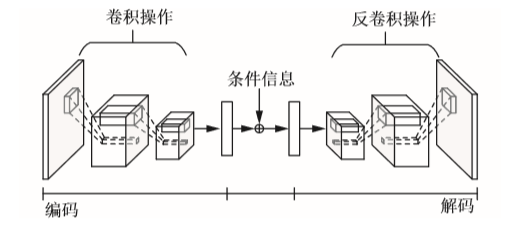
\includegraphics[width = 0.4\textwidth]{auto_encoder.png}
	\caption{基于自编码器的视频预测模型架构}
	\label{auto_encoder}
\end{figure}

自编码器架构下表现较好的是ConvLSTM,与LSTM不同,ConvLSTM在计算过程中用卷积操作代替了矩阵乘法,如公式~\ref{convLSTM}~所示,很好的利用卷积提取图像中的空间信息和利用LSTM提取时序信息。后来在ConvLSTM的基础上,又提出了训练代价更低,参数量更小的ConvGRU,在参数量和训练时间大大减少的前提下,精度能够得到基本保障。
\begin{equation}\label{convLSTM}
\begin{gathered}
$$
i_{t} = \sigma(W_{xi} \ast X_{t} + W_{hi} \ast H_{t-1} + W_{ci} \circ C_{t-1} + b_{i}) \\
f_{t} = \sigma(W_{xf} \ast X_{t} + W_{hf} \ast H_{t-1} + W_{cf} \circ C_{t-1} + b_{f})  \\
C_{t} = f_{t} \circ C_{t-1} + i_{t} \circ tanh(W_{xc} \ast X_{t} + W_{hc} \ast H_{t-1} + b_{c}) \\
o_{t} = \sigma(W_{xo} \ast X_{t} + W_{ho} \ast H_{t-1} + W_{oi} \circ C_{t-1} + b_{o})\\
H_{t} = o_{t} \circ tanh(C_{t})
$$
\end{gathered}
\end{equation}



% !Mode:: "TeX:UTF-8"

\chapter{基于卫星资料的初生对流像素级检测算法设计}[Example]


\section{基于卫星资料的初生对流数据集构建}[Number]

初生对流(CI)的物理定义为强对流天气发生前,大气各种物理量处于某种特殊的状态,换句话说初生对流的未来发展趋势应该是强对流。基于卫星资料的初生对流的标注工作,主要采用带有多通道时序的阈值法,通过当前时刻与未来15分钟和30分钟(即两帧图像)的卫星红外1(10.8um,IR1)、红外2(12um,IR2)与水汽(6.25um,WV)三个通道的信息,来标注初生对流的位置。其中共有8个阈值,其中F1到F8的分别为用以上信息设置的阈值限定指标,其中的物理意义代表了不同尺度下的云顶高度、云顶高度变化以及积云形态。其中满足任意7个阈值的像元,将会被标注为初生对流。

其中标注的阈值如下表~\ref{tb_threshold}~所示。

\begin{table}[h]
	\centering
	\label{tb_threshold}
	\caption{初生对流阈值指标}
	\begin{tabular}{c c c}
		\hline 序号 & CI预报指标 & 预报指标的判断阈值 \\
		\hline F1 & IR1亮温差 &	<0℃ \\
		 F2 &WV 与 IR1 亮温差 &	−35℃~−10℃ \\
		 F3 &IR2 与 IR1 亮温差 &	−25℃~−5℃\\
		 F4 &IR1 亮温变化率 &	<-4℃/(15 min) \\
		 F5 & IR1 亮温变化率&	∆T/(30 min)<∆T/(15 min) \\
		 F6 & IR1 亮温降低至 0℃的时间 &	<30 min \\
	 	 F7 &WV 与 IR1 亮温差变化率 &>3℃/(15 min) \\
		 F8 & IR2 与 IR1 亮温差变化率 &>2℃/(15 min) \\
		\hline 
	\end{tabular}
\end{table}

通过此多通道时序的阈值法,构造了2018年FY-4a卫星全国范围内的初生对流数据集,选取了其中对流出现较为频繁的6-10月的华南地区作为此项课题的数据集。数据集的输入数据为当前时刻t的卫星数据以及当前时刻前3帧的卫星数据序列,即t-15,t-30,t-45。数据集的输出数据为当前时刻t为基准标注的初生对流掩码图像。其中t时刻的初生对流掩码是利用上述多通道阈值法通过t时刻,t+15时刻,以及t+30时刻标注出来的。
以2018年7月15日为例,数据集一条数据可视化的效果如~\ref{tb_vis_dataset}~所示。

\begin{table}[h]
	\centering
	\label{tb_vis_dataset}
	\caption{多通道云图序列数据展示图}
	\begin{tabular}{c c c c c}
		\hline  通道 & t-45 & t-30 & t-15 & t \\
		\hline \\
		水汽通道WV &
		\begin{minipage}[b]{0.15\columnwidth}
			\centering
			\raisebox{-.5\height}{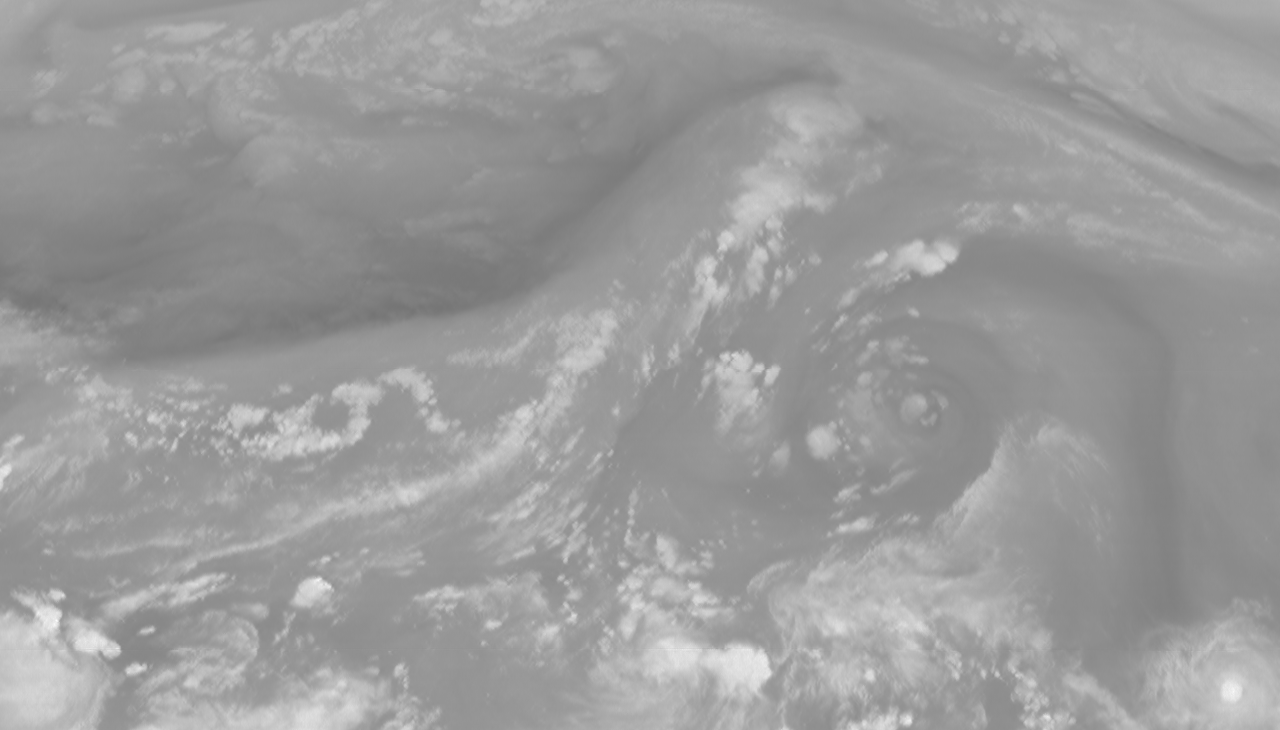
\includegraphics[width=\linewidth]{0000.png}}
		\end{minipage}&
		 \begin{minipage}[b]{0.15\columnwidth}
				 	\centering
				 	\raisebox{-.5\height}{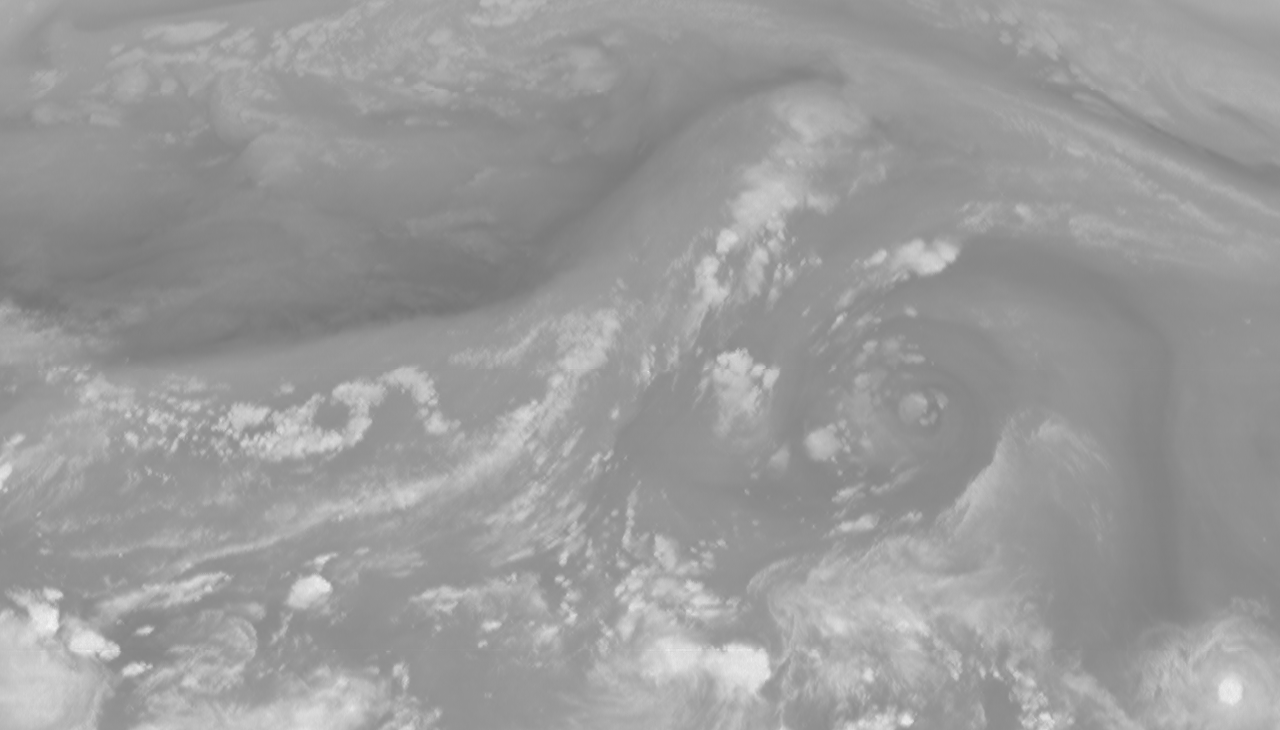
\includegraphics[width=\linewidth]{0000 (1).png}}
		 \end{minipage}&
		\begin{minipage}[b]{0.15\columnwidth}
		  	\centering
		  	\raisebox{-.5\height}{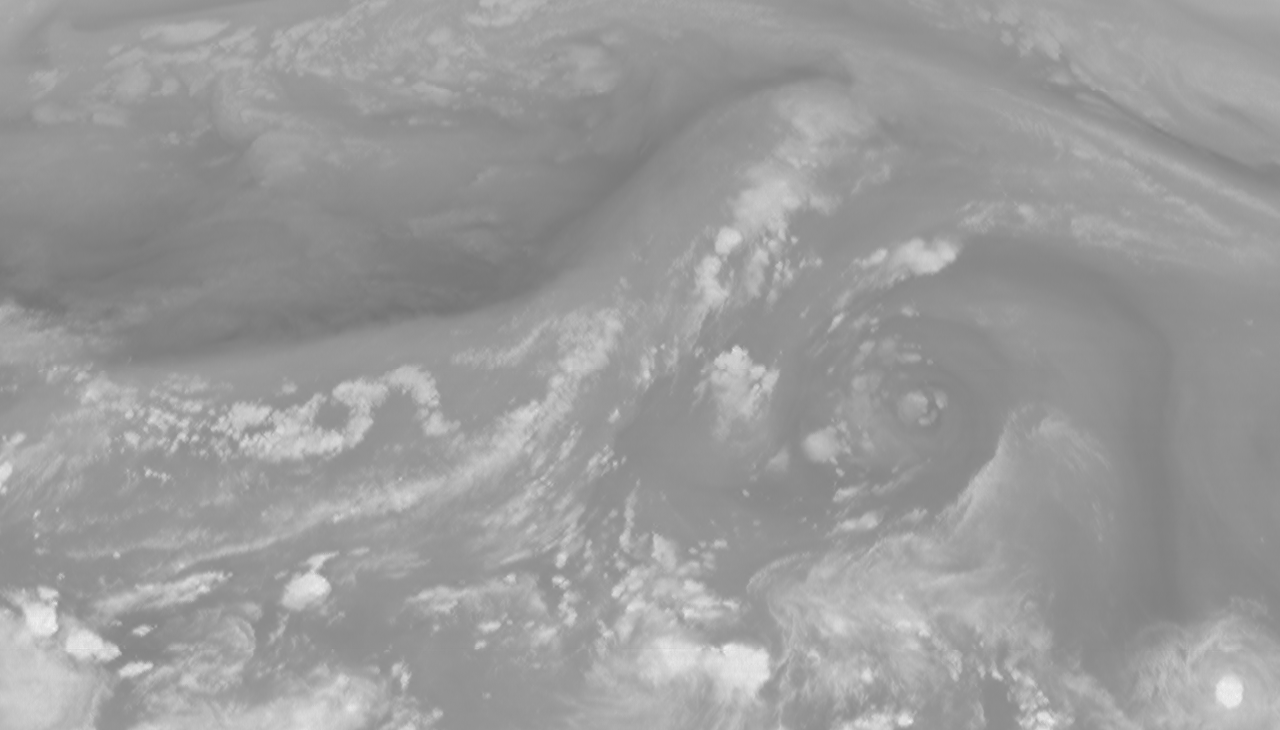
\includegraphics[width=\linewidth]{0000 (2).png}}
		\end{minipage}& 
		\begin{minipage}[b]{0.15\columnwidth}
		  	\centering
		  	\raisebox{-.5\height}{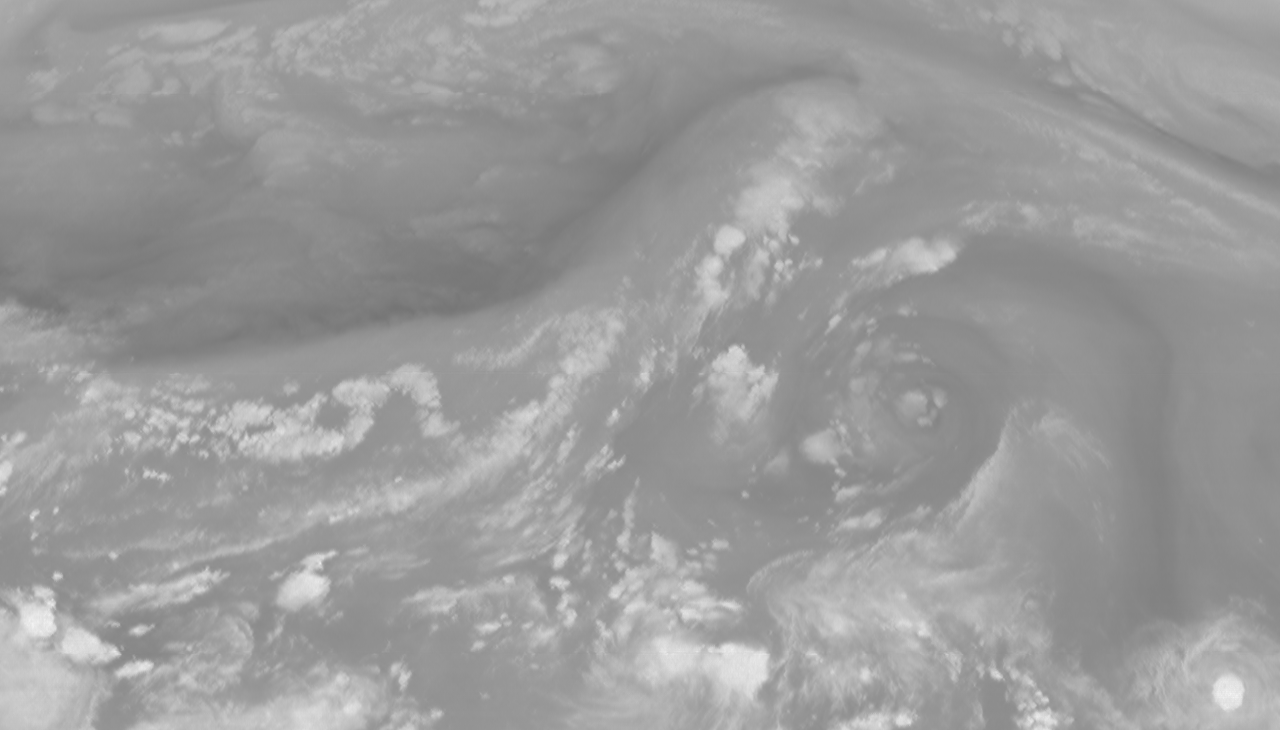
\includegraphics[width=\linewidth]{0000 (3).png}}
		\end{minipage}\\
	\\
			红外通道IR1 &
	\begin{minipage}[b]{0.15\columnwidth}
		\centering
		\raisebox{-.5\height}{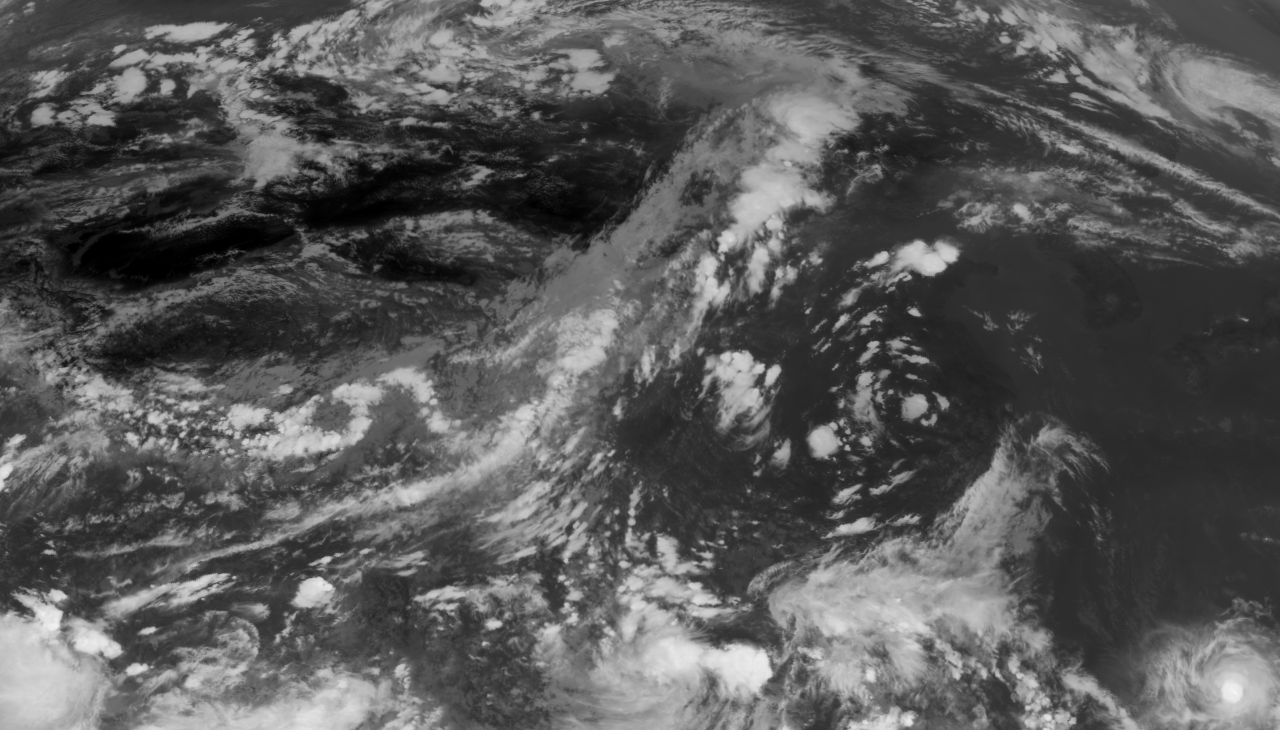
\includegraphics[width=\linewidth]{0001.png}}
	\end{minipage}&
	\begin{minipage}[b]{0.15\columnwidth}
		\centering
		\raisebox{-.5\height}{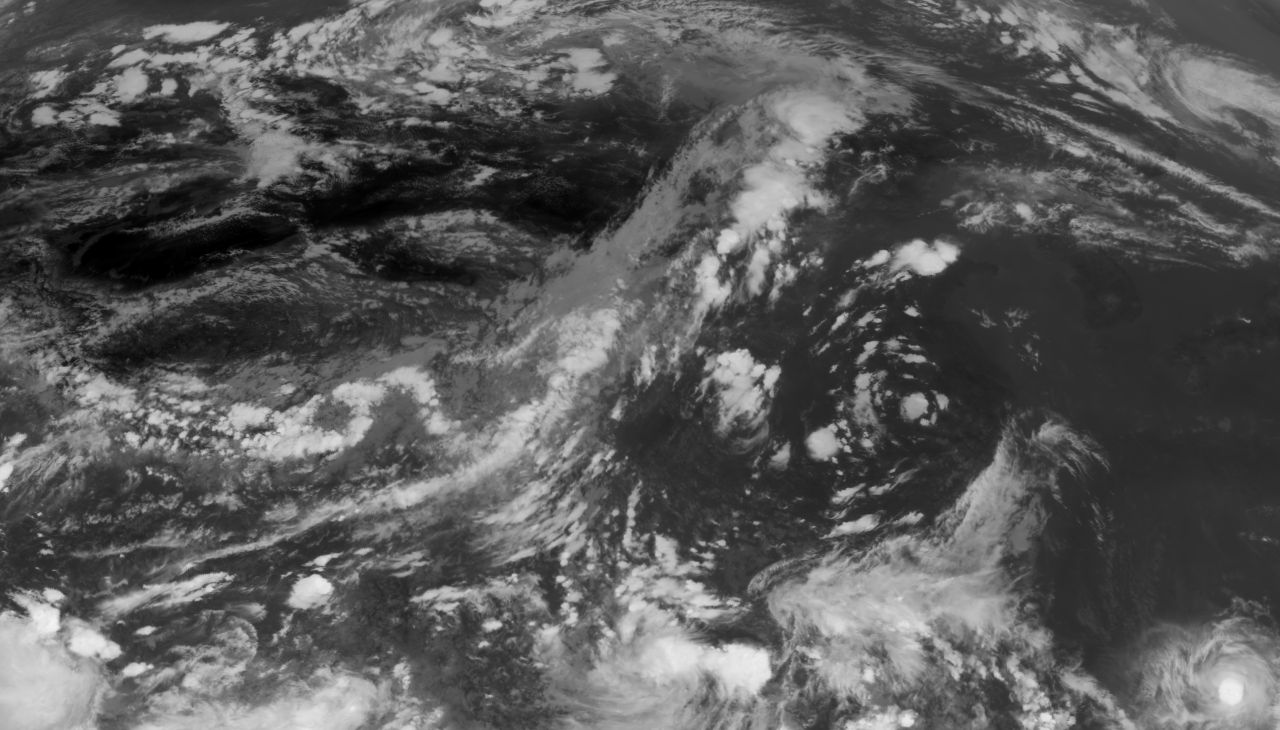
\includegraphics[width=\linewidth]{0001 (1).png}}
	\end{minipage}&
	\begin{minipage}[b]{0.15\columnwidth}
		\centering
		\raisebox{-.5\height}{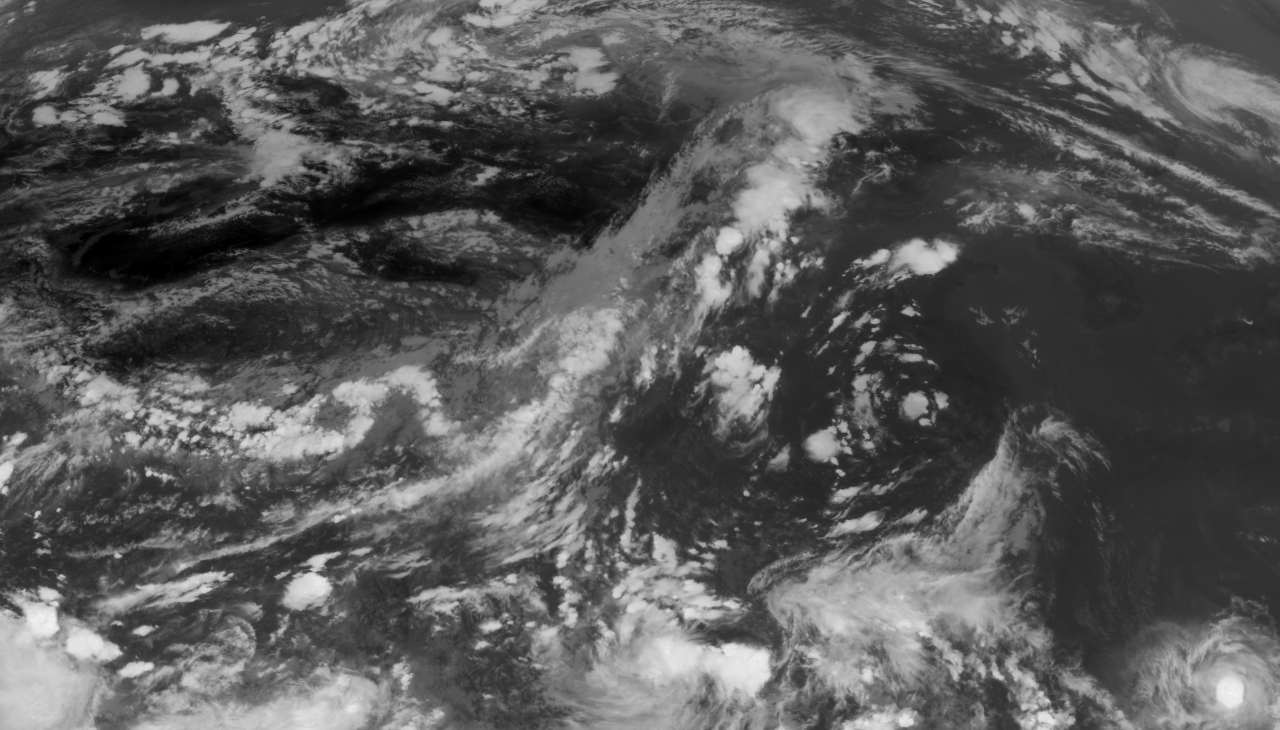
\includegraphics[width=\linewidth]{0001 (2).png}}
	\end{minipage}& 
	\begin{minipage}[b]{0.15\columnwidth}
		\centering
		\raisebox{-.5\height}{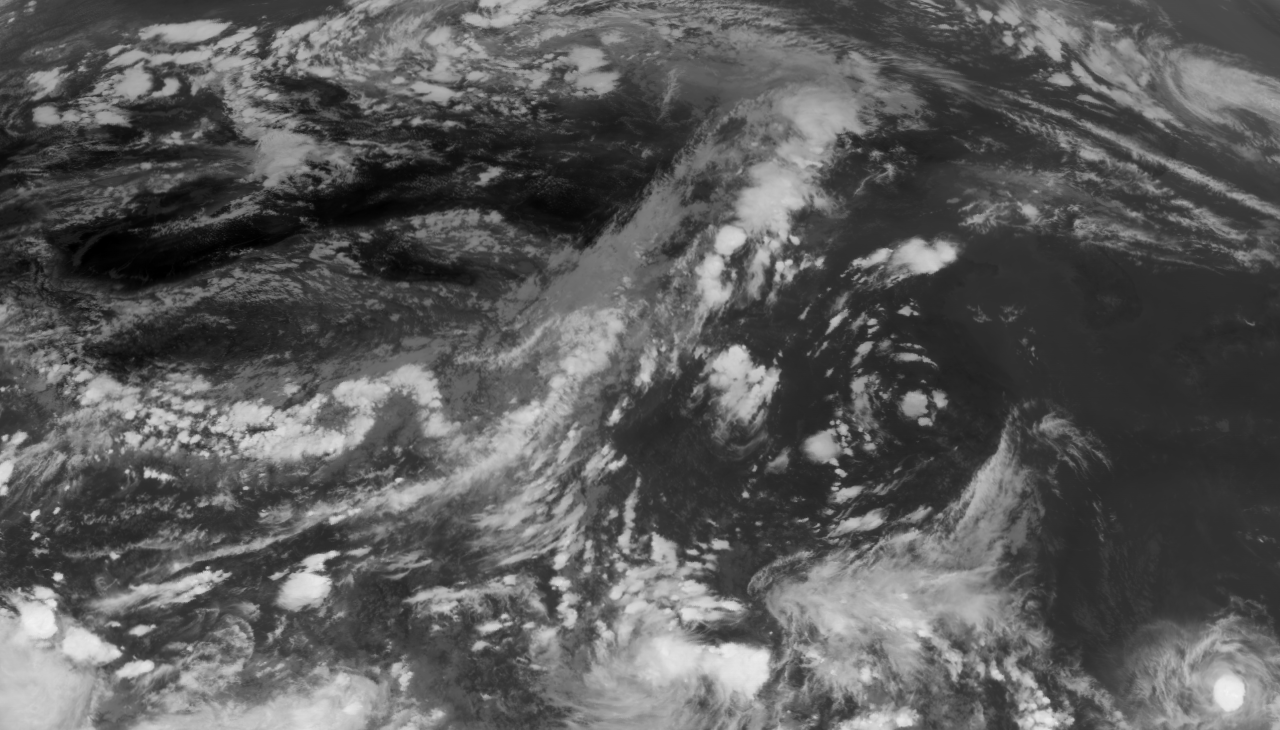
\includegraphics[width=\linewidth]{0001 (3).png}}
	\end{minipage}\\
	\\
			红外通道IR2 &
	\begin{minipage}[b]{0.15\columnwidth}
		\centering
		\raisebox{-.5\height}{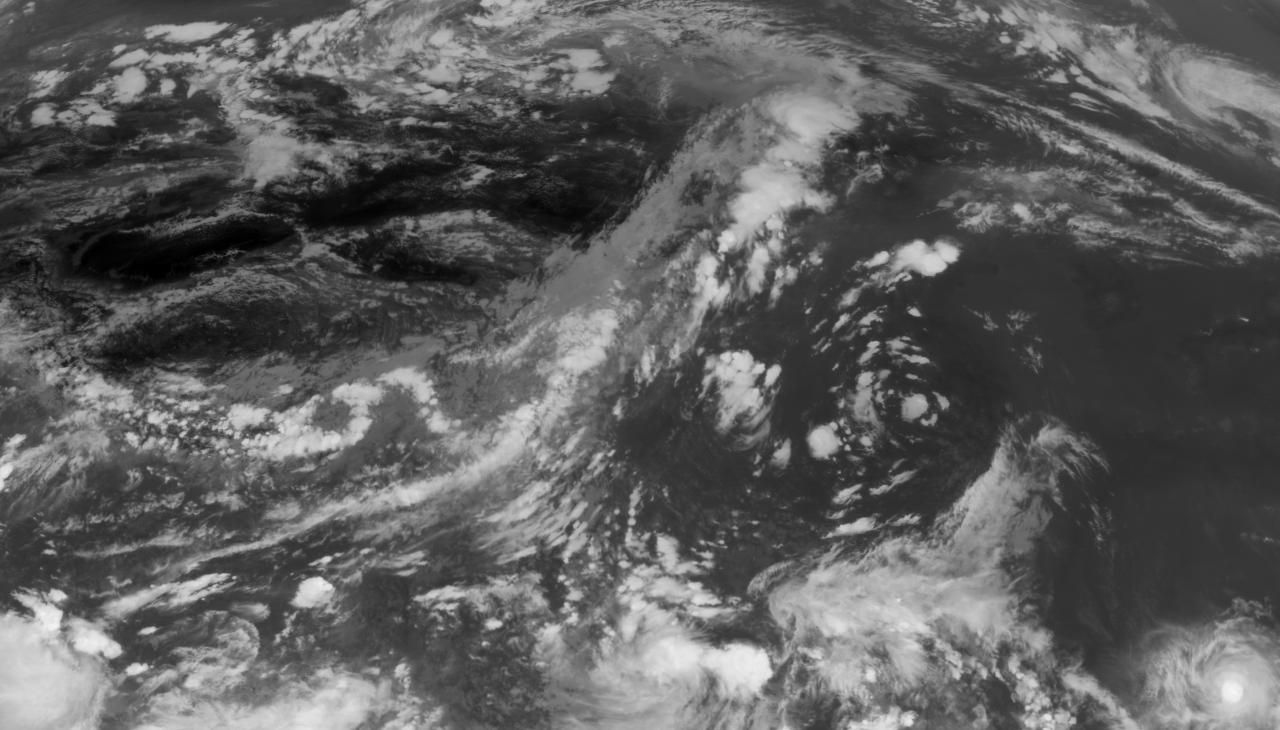
\includegraphics[width=\linewidth]{0002.png}}
	\end{minipage}&
	\begin{minipage}[b]{0.15\columnwidth}
		\centering
		\raisebox{-.5\height}{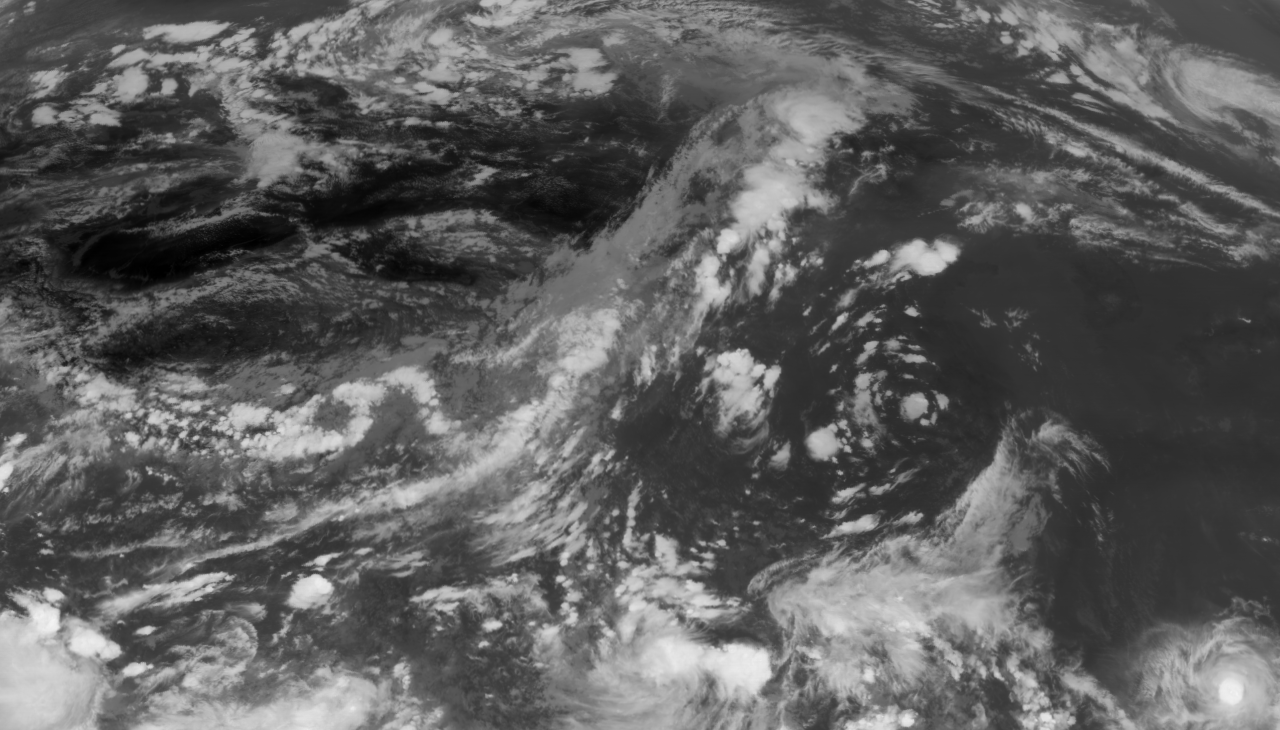
\includegraphics[width=\linewidth]{0002 (1).png}}
	\end{minipage}&
	\begin{minipage}[b]{0.15\columnwidth}
		\centering
		\raisebox{-.5\height}{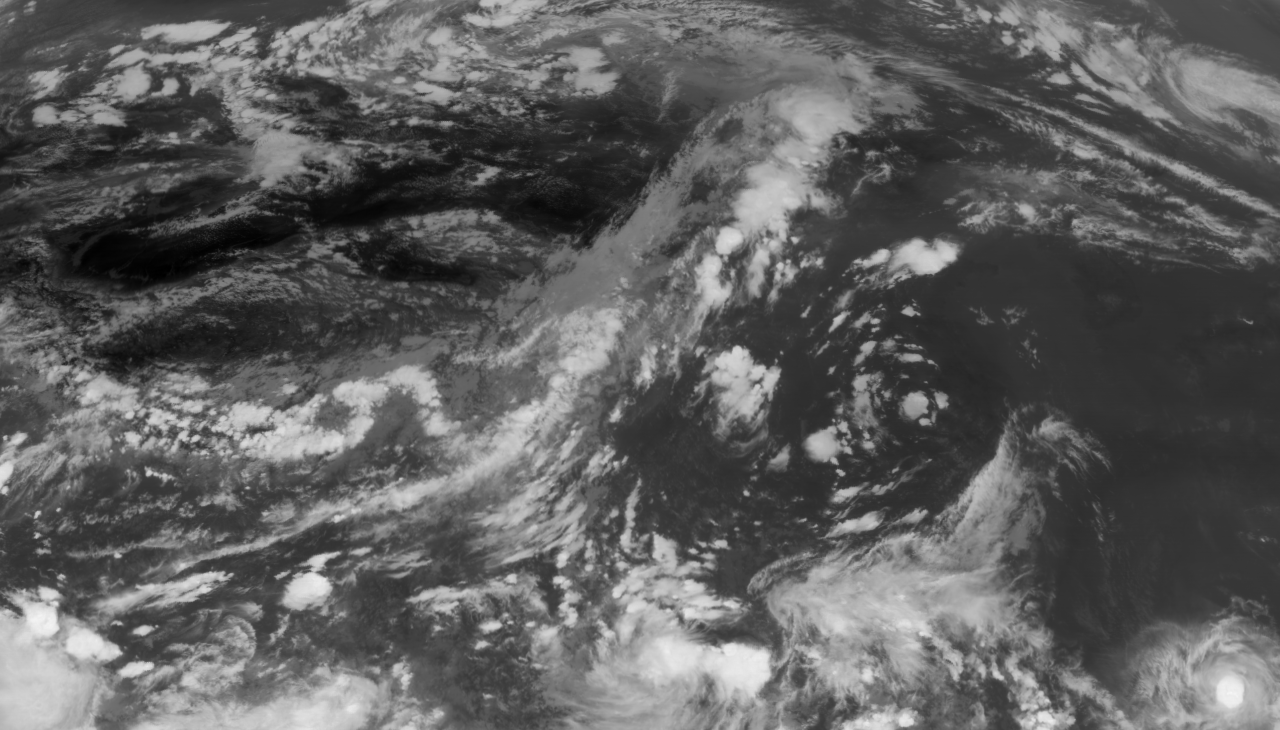
\includegraphics[width=\linewidth]{0002 (2).png}}
	\end{minipage}& 
	\begin{minipage}[b]{0.15\columnwidth}
		\centering
		\raisebox{-.5\height}{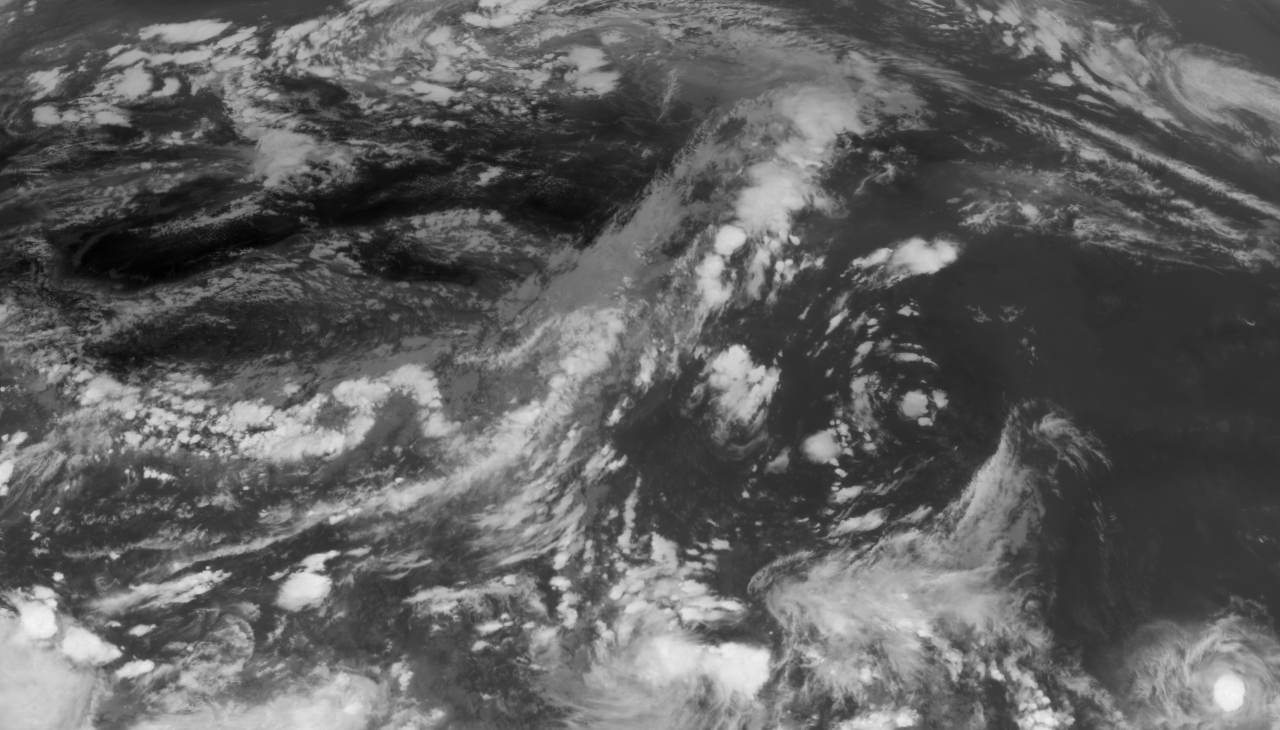
\includegraphics[width=\linewidth]{0002 (3).png}}
	\end{minipage}\\
	\\
 \hline
	\end{tabular}
\end{table}
\begin{table}[h]
	\centering
	\label{tb_vis_dataset_label}
	\caption{初生对流可视化类别标注即掩码展示图}
	\begin{tabular}{c c}
		\hline 可视化类别标注结果 & 类别标注掩码 \\
		\hline \\
		\begin{minipage}[b]{0.42\columnwidth}
			\centering
			\raisebox{-.5\height}{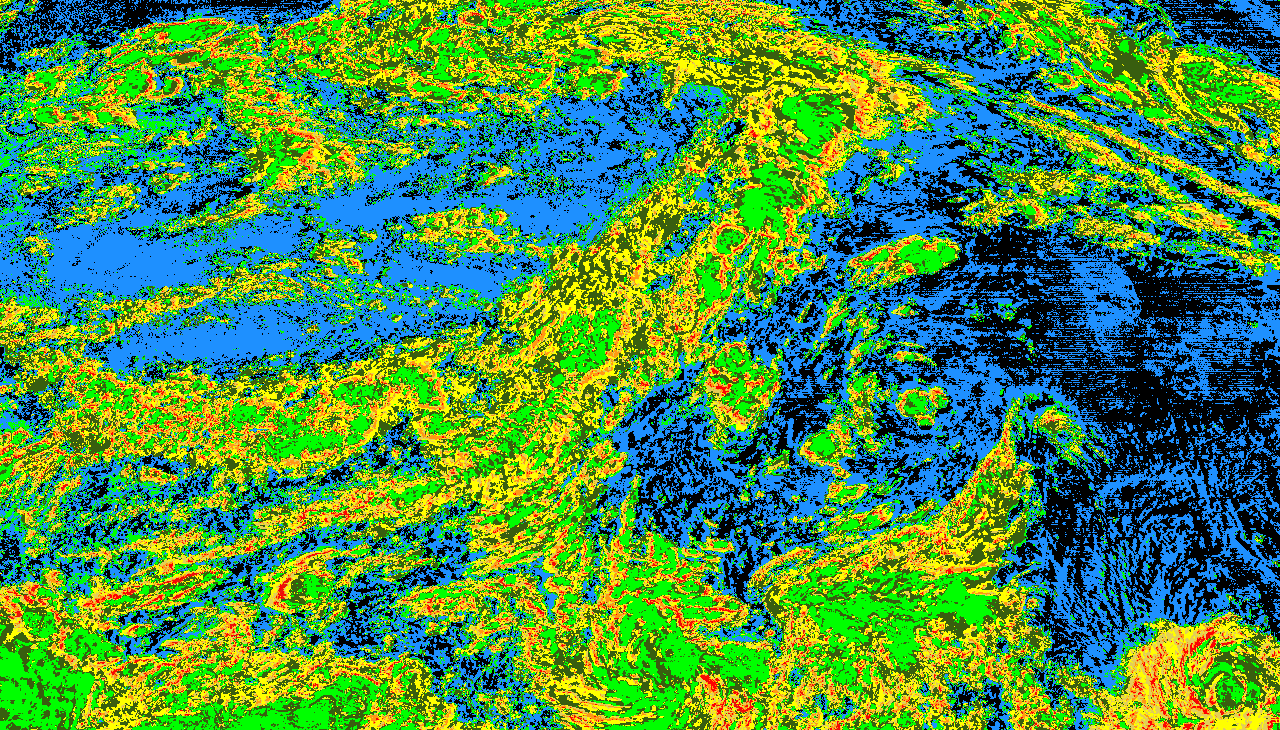
\includegraphics[width=\linewidth]{000mp.png}}
		\end{minipage}&
		\begin{minipage}[b]{0.42\columnwidth}
			\centering
			\raisebox{-.5\height}{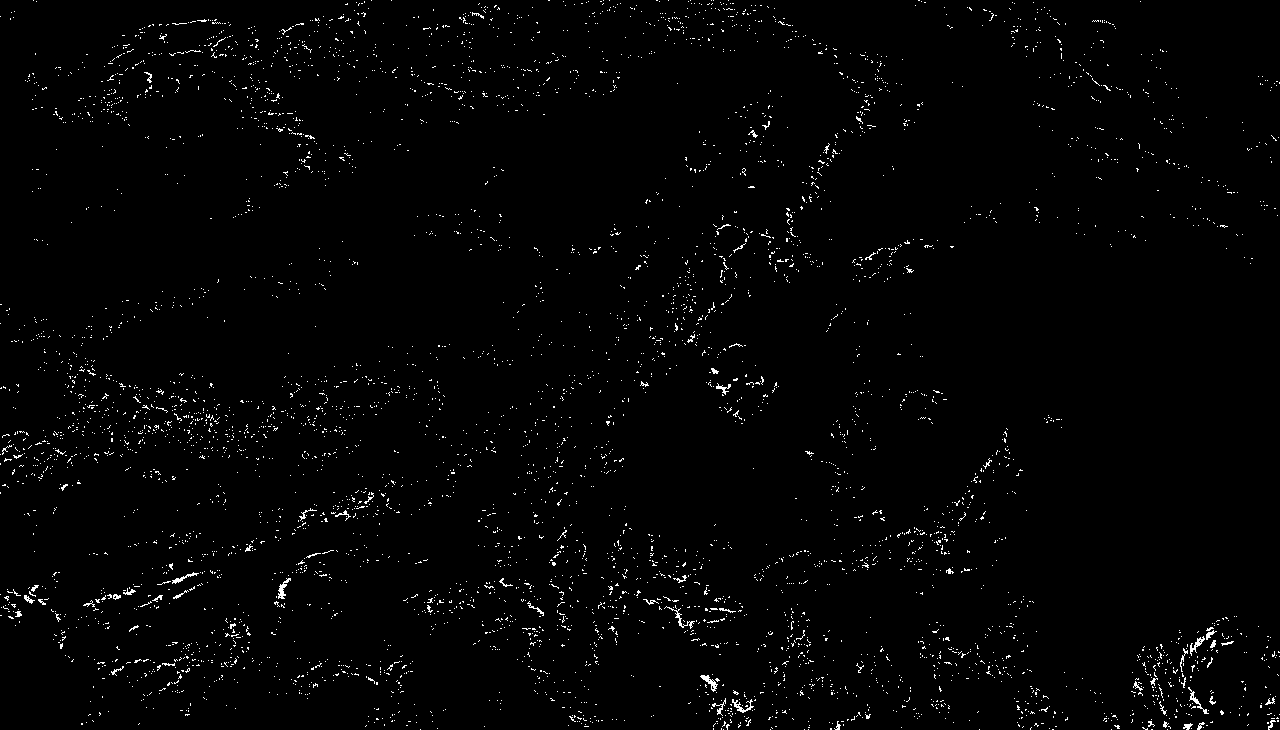
\includegraphics[width=\linewidth]{000lb.png}}
		\end{minipage} \\
	\\
	\hline
	\end{tabular}
\end{table}

经过统计分析,每张类别标注图像中存在初生对流的平均比率为0.79\%,平均每张图像存在7457个初生对流样本像元。可见其中的类别比例严重失衡。

\subsection{融合DenseConnection的RCNN模型结构}

对于像素级分类这一问题,本课题采用了RCNN模型作为基础模型进行初生对流的预测工作。初生对流多存在于云团系的边缘附近,因此要判识初生对流,模型至少需要一个像元附近的周围的像元来判别是否在云团边缘,从而更好的判识初生对流。一般初生对流所联通的区域很小,通常仅仅是一个或者几个像元相联通,而其中一个像元单独存在且不连通的样本占绝大多数。因此本课题所采用的模型是能够擅长处理像素级分类的循环卷积神经网络RCNN。

RCNN模型是逐步缩小检测范围的多层卷积神经网络结构,相比CNN能够复用不同尺度特征,有效提取像元的空间信息。RCNN模型相比于语义分割模型(Unet、Deeplab)等对于处理单个像元分类的任务要更加优秀,语义分割模型更擅长处理大范围联通样本分类问题。

基础的RCNN模型如图~\ref{RCNN_model}~所示:

\begin{figure}[h]
	\centering
	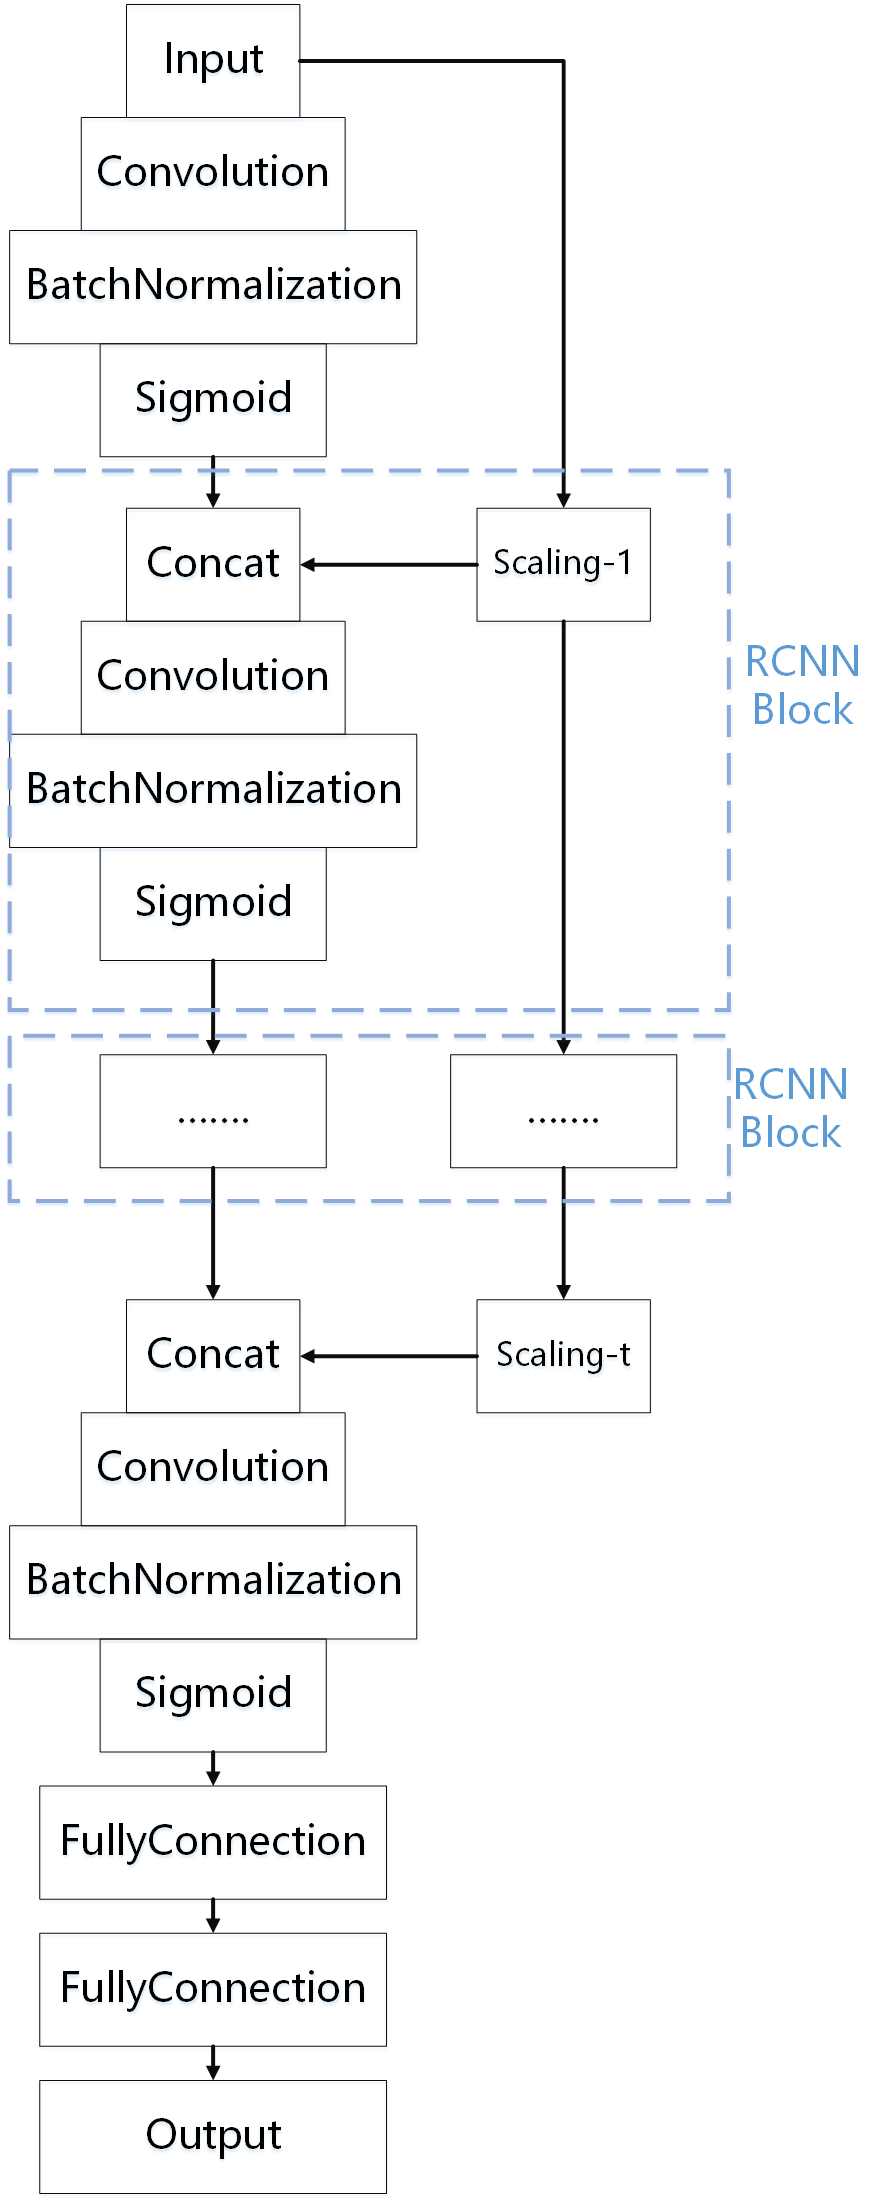
\includegraphics[width = 0.4\textwidth]{RCNN模型框架.png}
	\caption{RCNN模型框架}
	\label{RCNN_model}
\end{figure}

RCNN模型中基本的结构为RCNN Block,由一次2D卷积一次批标准化以及一层激活函数组成。RCNN Block每层所接受的输入为上一层的结果以及原始图像缩放后经过通道连接的张量。由~\ref{feature_importance}~,可见其中对于越靠近像元中心的像元,其RCNN的模型对其的附加的权重就越大。

\begin{figure}[h]
	\centering
	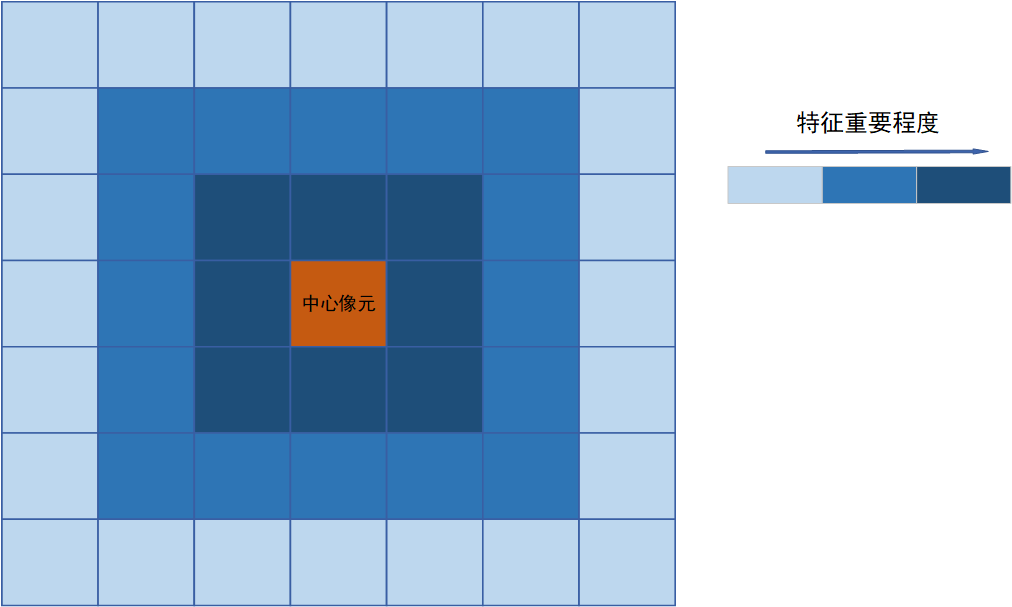
\includegraphics[width = 0.4\textwidth]{特征重要程度.png}
	\caption{特征重要程度}
	\label{feature_importance}
\end{figure}

然而真实情况下单独依靠像元中心并不能判识初生对流,甚至无法判识云团边缘。不同层级的RCNN卷积核用于提取不同尺度的特征,随着层数加深卷积核所提取的特征所概况的空间信息越少,而很多情况下初生对流所依赖的特征所属于较初始的低阶特征,因此这里引入DenseConnection结构,每次卷积都保留上一层所有的特征图,对特征依次传递保留,如~\ref{Dense_RCNN_model}~所示。

\begin{figure}[h]
	\centering
	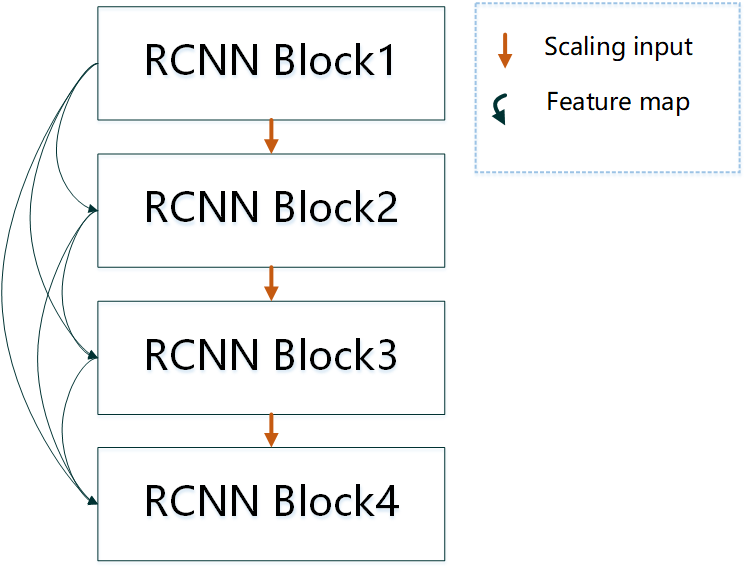
\includegraphics[width = 0.4\textwidth]{block.png}
	\caption{Dense-RCNN连接结构}
	\label{Dense_RCNN_model}
\end{figure}

Dense-RCNN相较于RCNN精度有较为明显的提升,DenseConnection来源于DenseNet,DenseNet的后序之作SENet是基于DenseNet在深度卷积神经网络中的数据集中取得了更好的效果。SE结构在DenseConnection上加以改进,上一层特征通道的简单叠加替换为了附加权重的特征叠加,通过一层特征选择支流给特征赋予权重。SE-RCNN相比Dense-RCNN结果的精度又有微弱提升。

\begin{figure}[h]
	\centering
	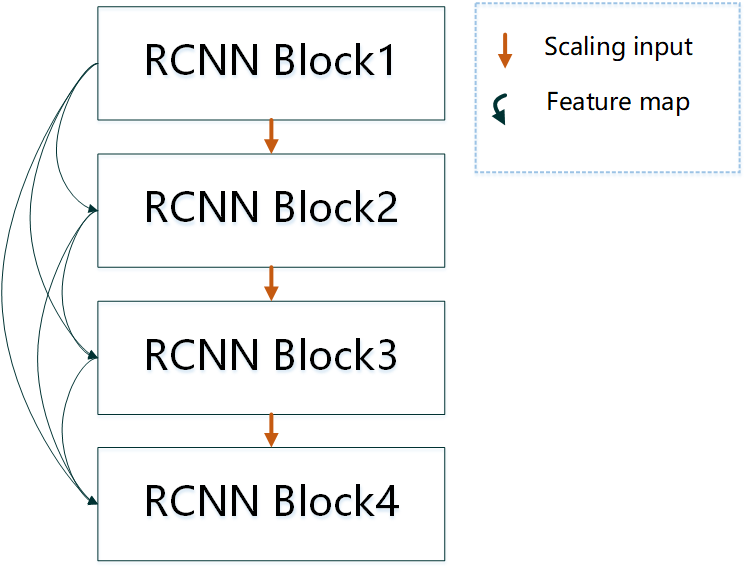
\includegraphics[width = 0.4\textwidth]{block.png}
	\caption{Dense-RCNN连接结构}
	\label{Dense_RCNN_model}
\end{figure}

\backmatter
% !Mode:: "TeX:UTF-8" 
\begin{conclusions}

学位论文的结论作为论文正文的最后一章单独排写,但不加章标题序号。

结论应是作者在学位论文研究过程中所取得的创新性成果的概要总结,不能与摘要混为一谈。博士学位论文结论应包括论文的主要结果、创新点、展望三部分,在结论中应概括论文的核心观点,明确、客观地指出本研究内容的创新性成果(含新见解、新观点、方法创新、技术创新、理论创新),并指出今后进一步在本研究方向进行研究工作的展望与设想。对所取得的创新性成果应注意从定性和定量两方面给出科学、准确的评价,分(1)、(2)、(3)…条列出,宜用“提出了”、“建立了”等词叙述。

\end{conclusions}
   % 结论
\bibliographystyle{hithesis} %如果没有参考文献时候
\bibliography{reference}
%%%%%%%%%%%%%%%%%%%%%%%%%%%%%%%%%%%%%%%%%%%%%%%%%%%%%%%%%%%%%%%%%%%%%%%%%%%%%%%% 
%-- 注意:以下本硕博、博后书序不一致 --%
%%%%%%%%%%%%%%%%%%%%%%%%%%%%%%%%%%%%%%%%%%%%%%%%%%%%%%%%%%%%%%%%%%%%%%%%%%%%%%%% 
%硕博书序
%%%%%%%%%%%%%%%%%%%%%%%%%%%%%%%%%%%%%%%%%%%%%%%%%%%%%%%%%%%%%%%%%%%%%%%%%%%%%%%% 
\begin{appendix}%附录
%% -*-coding: utf-8 -*-
%%%%%%%%%%%%%%%%%%%%%%%%%%%%%%%%%%%%%%%%%%%%%%%%%%%%%%%%%
\chapter{带章节的附录}[Full Appendix]%
完整的附录内容,包含章节,公式,图表等

%%%%%%%%%%%%%%%%%%%%%%%%%%%%%%%%%%%%%%%%%%%%%%%%%%%%%%%%%
\section{附录节的内容}[Section in Appendix]
这是附录的节的内容

附录中图的示例:
\begin{figure}[htbp]
\centering
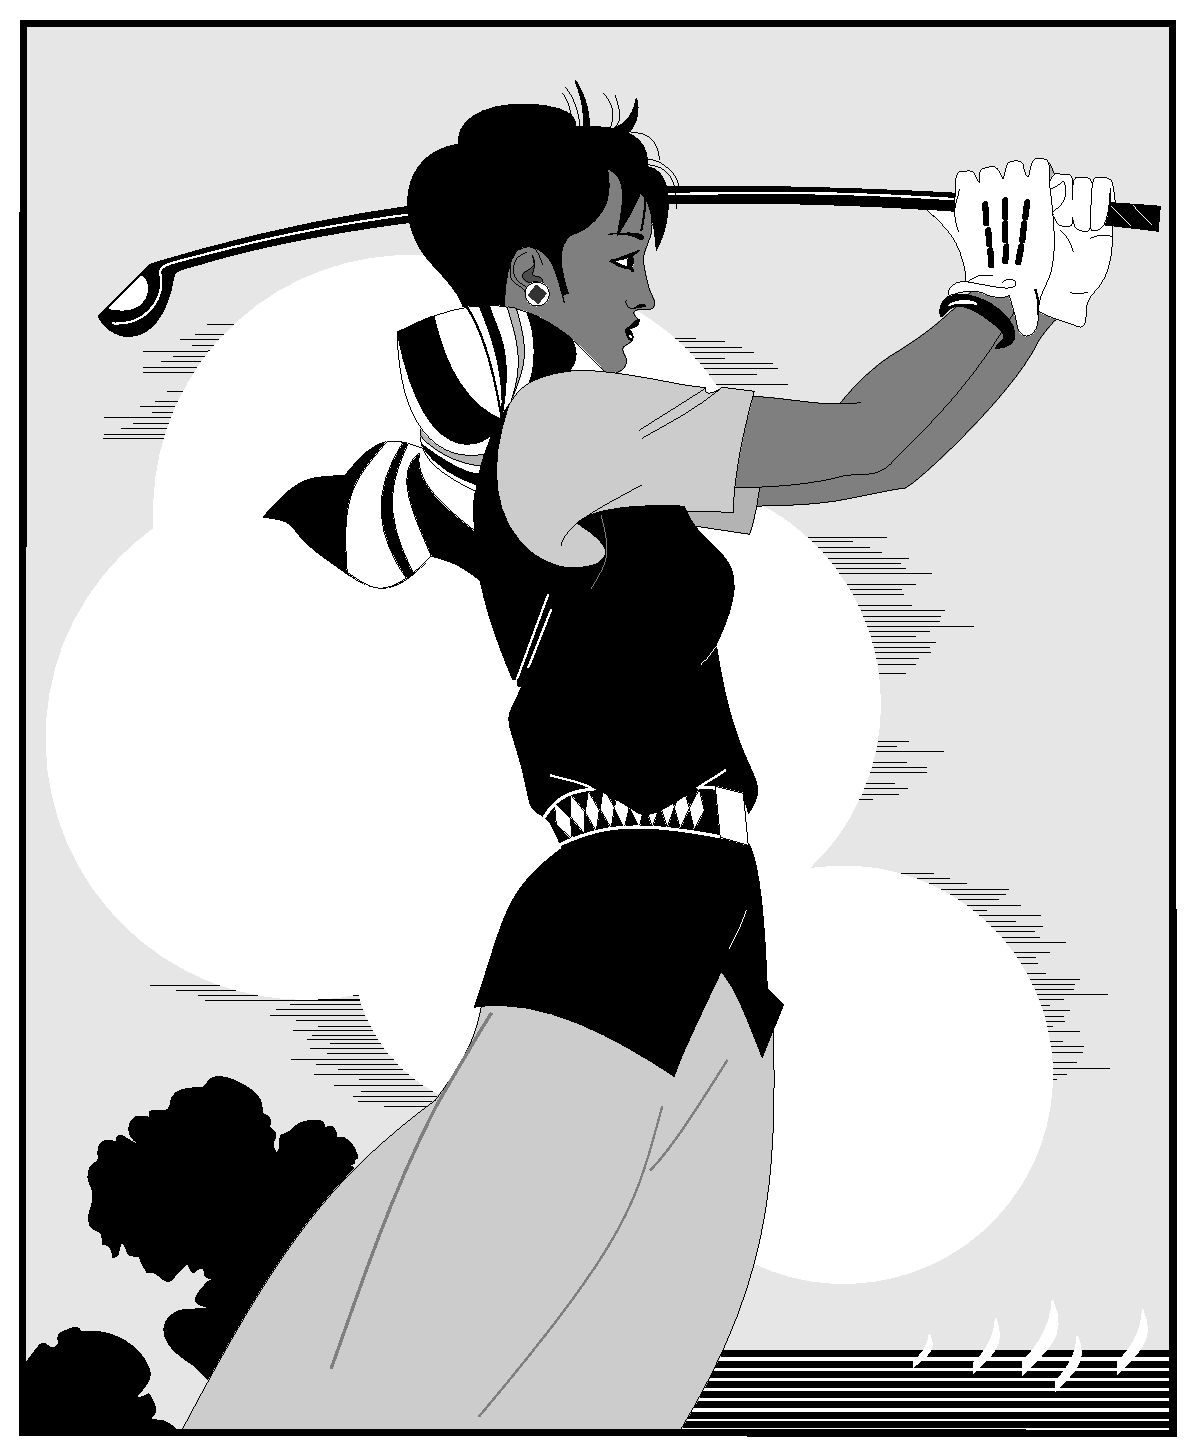
\includegraphics[width = 0.4\textwidth]{golfer}
%\bicaption[golfer5]{}{\xiaosi[0]打高尔夫球的人}{Fig.$\!$}{The person playing golf}\vspace{-1em}
\caption{\xiaosi[0]打高尔夫球的人}
\end{figure}

附录中公式的示例:
\begin{align}
a & = b \times c \\
E & = m c^2
\label{eq}
\end{align}

\chapter{这个星球上最好的免费Linux软件列表}[List of the Best Linux Software in our Planet]
\section{系统}

\href{http://fvwm.org/}{FVWM 自从上世纪诞生以来,此星球最强大的窗口管理器。}
推荐基于FVWM的桌面设计hifvwm:\href{https://github.com/dustincys/hifvwm}{https://github.com/dustincys/hifvwm}。

\subsection{hifvwm的优点}

\begin{enumerate}
	\item 即使打开上百个窗口也不会“蒙圈”。计算机性能越来越强大,窗口任务的管理必须要升级到打怪兽级别。
	\item 自动同步Bing搜索主页的壁纸。每次电脑开机,午夜零点自动更新,用户
		也可以手动更新,从此审美再也不疲劳。
	\item 切换窗口自动聚焦到最上面的窗口。使用键盘快捷键切换窗口时候,减少
		操作过程,自动聚焦到目标窗口。这一特性是虚拟窗口必须的人性化设
		计。
	\item 类似window右下角的功能的最小化窗口来显示桌面的功能此处类似
		win7/win10,实现在一个桌面之内操作多个任务。
	\item 任务栏结合标题栏。采用任务栏和标题栏结合,节省空间。
	\item 同类窗口切换。可以在同类窗口之内类似alt-tab的方式切换。
	\item ……
\end{enumerate}

\section{其他}

\href{https://github.com/goldendict/goldendict}{goldendict 星球最强大的桌面字典。}

\href{https://github.com/yarrick/iodine}{iodine,“HIT-WLAN + 锐捷”时代的福音。}

\href{http://www.aircrack-ng.org/}{aircrack,Wifi“安全性评估”工具。}

\href{https://www.ledger-cli.org/}{ledger,前“金融区块链”时代最好的复式记账系统。}

\href{https://orgmode.org/}{orgmode,最强大的笔记系统,从来没有之一。}

\href{https://www.jianguoyun.com/}{坚果云,国内一款支持WebDav的云盘系统,国内真正的云盘没有之一。}

\href{http://www.mutt.org/}{mutt, ``All mail clients suck. This one just sucks less.''}

\section{vim}
实现中英文每一句一行,以及实现每一句折叠断行的简单正则式,tex源码更加乖乖。
\begin{lstlisting}
vnoremap <leader>fae J:s/[.!?]\zs\s\+/\="\r".matchstr(getline('.'), '^\s*')/g<CR>
vnoremap <leader>fac J:s/[。!?]/\=submatch(0)."\n".matchstr(getline('.'), '^\s*')/g<CR>
vnoremap <leader>fle :!fmt -80 -s<CR>
\end{lstlisting}

\end{appendix}
%% !Mode:: "TeX:UTF-8" 
\begin{publication}
\noindent\textbf{发表的相关论文}
\begin{publist}
\item	XXX,XXX. Static Oxidation Model of Al-Mg/C Dissipation Thermal Protection Materials[J]. Rare Metal Materials and Engineering, 2010, 39(Suppl. 1): 520-524.(SCI~收录,IDS号为~669JS,IF=0.16)
\item XXX,XXX. 精密超声振动切削单晶铜的计算机仿真研究[J]. 系统仿真学报,2007,19(4):738-741,753.(EI~收录号:20071310514841)
\item XXX,XXX. 局部多孔质气体静压轴向轴承静态特性的数值求解[J]. 摩擦学学报,2007(1):68-72.(EI~收录号:20071510544816)
\item XXX,XXX. 硬脆光学晶体材料超精密切削理论研究综述[J]. 机械工程学报,2003,39(8):15-22.(EI~收录号:2004088028875)
\item XXX,XXX. 基于遗传算法的超精密切削加工表面粗糙度预测模型的参数辨识以及切削参数优化[J]. 机械工程学报,2005,41(11):158-162.(EI~收录号:2006039650087)
\item XXX,XXX. Discrete Sliding Mode Cintrok with Fuzzy Adaptive Reaching Law on 6-PEES Parallel Robot[C]. Intelligent System Design and Applications, Jinan, 2006: 649-652.(EI~收录号:20073210746529)
\end{publist}

\noindent\textbf{(二)申请及已获得的专利(无专利时此项不必列出)}
\begin{publist}
\item XXX,XXX. 一种温热外敷药制备方案:中国,88105607.3[P]. 1989-07-26.
\end{publist}

\noindent\textbf{(三)参与的科研项目及获奖情况}
\begin{publist}
\item	XXX,XXX. XX~气体静压轴承技术研究, XX~省自然科学基金项目.课题编号:XXXX.
\item XXX,XXX. XX~静载下预应力混凝土房屋结构设计统一理论. 黑江省科学技术二等奖, 2007.
\end{publist}
%\vfill
%\hangafter=1\hangindent=2em\noindent
%\setlength{\parindent}{2em}
\end{publication}
    % 所发文章
%\begin{ceindex}
  %如果想要手动加索引,注释掉以下这一样,用wordlist环境
\printsubindex*
\end{ceindex}
    % 索引, 根据自己的情况添加或者不添加,选择自动添加或者手工添加。
\authorization %授权
%\authorization[saomiao.pdf] %添加扫描页的命令,与上互斥
%% !Mode:: "TeX:UTF-8"
\begin{acknowledgements}

Thank to \hithesis\ !


\end{acknowledgements}
 %致谢
%% !Mode:: "TeX:UTF-8" 

\begin{resume}
XXXX~年~XX~月~XX~日出生于~XXXX。

XXXX~年~XX~月考入~XX~大学~XX~院(系)XX~专业,XXXX~年~XX~月本科毕业并获得~XX~学学士学位。

XXXX~年~XX~月------XXXX~年~XX~月在~XX~大学~XX~院(系)XX~学科学习并获得~XX~学硕士学位。

XXXX~年~XX~月------XXXX~年~XX~月在~XX~大学~XX~院(系)XX~学科学习并获得~XX~学博士学位。

获奖情况:如获三好学生、优秀团干部、X~奖学金等(不含科研学术获奖)。

工作经历:

\textbf{( 除全日制硕士生以外,其余学生均应增列此项。个人简历一般应包含教育经历和工作经历。)}
\end{resume}
          % 博士学位论文有个人简介
%%%%%%%%%%%%%%%%%%%%%%%%%%%%%%%%%%%%%%%%%%%%%%%%%%%%%%%%%%%%%%%%%%%%%%%%%%%%%%%% 
%本科书序为:
%%%%%%%%%%%%%%%%%%%%%%%%%%%%%%%%%%%%%%%%%%%%%%%%%%%%%%%%%%%%%%%%%%%%%%%%%%%%%%%% 
% \authorization %授权
% % \authorization[saomiao.pdf] %添加扫描页的命令,与上互斥
% % !Mode:: "TeX:UTF-8"
\begin{acknowledgements}

Thank to \hithesis\ !


\end{acknowledgements}
 %致谢
% \begin{appendix}%附录
% \chapter{外文资料原文}
\label{cha:engorg}

\title{The title of the English paper}

\textbf{Abstract:} As one of the most widely used techniques in operations
research, \emph{ mathematical programming} is defined as a means of maximizing a
quantity known as \emph{bjective function}, subject to a set of constraints
represented by equations and inequalities. Some known subtopics of mathematical
programming are linear programming, nonlinear programming, multiobjective
programming, goal programming, dynamic programming, and multilevel
programming$^{[1]}$.

It is impossible to cover in a single chapter every concept of mathematical
programming. This chapter introduces only the basic concepts and techniques of
mathematical programming such that readers gain an understanding of them
throughout the book$^{[2,3]}$.


\section{Single-Objective Programming}
The general form of single-objective programming (SOP) is written
as follows,
\begin{equation}\tag*{(123)} % 如果附录中的公式不想让它出现在公式索引中,那就请
                             % 用 \tag*{xxxx}
\left\{\begin{array}{l}
\max \,\,f(x)\\[0.1 cm]
\mbox{subject to:} \\ [0.1 cm]
\qquad g_j(x)\le 0,\quad j=1,2,\cdots,p
\end{array}\right.
\end{equation}
which maximizes a real-valued function $f$ of
$x=(x_1,x_2,\cdots,x_n)$ subject to a set of constraints.

\newtheorem{mpdef}{Definition}[chapter]
\begin{mpdef}
In SOP, we call $x$ a decision vector, and
$x_1,x_2,\cdots,x_n$ decision variables. The function
$f$ is called the objective function. The set
\begin{equation}\tag*{(456)} % 这里同理,其它不再一一指定。
S=\left\{x\in\Re^n\bigm|g_j(x)\le 0,\,j=1,2,\cdots,p\right\}
\end{equation}
is called the feasible set. An element $x$ in $S$ is called a
feasible solution.
\end{mpdef}

\newtheorem{mpdefop}[mpdef]{Definition}
\begin{mpdefop}
A feasible solution $x^*$ is called the optimal
solution of SOP if and only if
\begin{equation}
f(x^*)\ge f(x)
\end{equation}
for any feasible solution $x$.
\end{mpdefop}

One of the outstanding contributions to mathematical programming was known as
the Kuhn-Tucker conditions\ref{eq:ktc}. In order to introduce them, let us give
some definitions. An inequality constraint $g_j(x)\le 0$ is said to be active at
a point $x^*$ if $g_j(x^*)=0$. A point $x^*$ satisfying $g_j(x^*)\le 0$ is said
to be regular if the gradient vectors $\nabla g_j(x)$ of all active constraints
are linearly independent.

Let $x^*$ be a regular point of the constraints of SOP and assume that all the
functions $f(x)$ and $g_j(x),j=1,2,\cdots,p$ are differentiable. If $x^*$ is a
local optimal solution, then there exist Lagrange multipliers
$\lambda_j,j=1,2,\cdots,p$ such that the following Kuhn-Tucker conditions hold,
\begin{equation}
\label{eq:ktc}
\left\{\begin{array}{l}
    \nabla f(x^*)-\sum\limits_{j=1}^p\lambda_j\nabla g_j(x^*)=0\\[0.3cm]
    \lambda_jg_j(x^*)=0,\quad j=1,2,\cdots,p\\[0.2cm]
    \lambda_j\ge 0,\quad j=1,2,\cdots,p.
\end{array}\right.
\end{equation}
If all the functions $f(x)$ and $g_j(x),j=1,2,\cdots,p$ are convex and
differentiable, and the point $x^*$ satisfies the Kuhn-Tucker conditions
(\ref{eq:ktc}), then it has been proved that the point $x^*$ is a global optimal
solution of SOP.

\subsection{Linear Programming}
\label{sec:lp}

If the functions $f(x),g_j(x),j=1,2,\cdots,p$ are all linear, then SOP is called
a {\em linear programming}.

The feasible set of linear is always convex. A point $x$ is called an extreme
point of convex set $S$ if $x\in S$ and $x$ cannot be expressed as a convex
combination of two points in $S$. It has been shown that the optimal solution to
linear programming corresponds to an extreme point of its feasible set provided
that the feasible set $S$ is bounded. This fact is the basis of the {\em simplex
  algorithm} which was developed by Dantzig as a very efficient method for
solving linear programming.
\begin{table}[ht]
\centering
  \centering
  \caption*{Table~1\hskip1em This is an example for manually numbered table, which
    would not appear in the list of tables}
  \label{tab:badtabular2}
  \begin{tabular}[c]{|m{1.5cm}|c|c|c|c|c|c|}\hline
    \multicolumn{2}{|c|}{Network Topology} & \# of nodes &
    \multicolumn{3}{c|}{\# of clients} & Server \\\hline
    GT-ITM & Waxman Transit-Stub & 600 &
    \multirow{2}{2em}{2\%}&
    \multirow{2}{2em}{10\%}&
    \multirow{2}{2em}{50\%}&
    \multirow{2}{1.2in}{Max. Connectivity}\\\cline{1-3}
    \multicolumn{2}{|c|}{Inet-2.1} & 6000 & & & &\\\hline
    & \multicolumn{2}{c|}{ABCDEF} &\multicolumn{4}{c|}{} \\\hline
\end{tabular}
\end{table}

Roughly speaking, the simplex algorithm examines only the extreme points of the
feasible set, rather than all feasible points. At first, the simplex algorithm
selects an extreme point as the initial point. The successive extreme point is
selected so as to improve the objective function value. The procedure is
repeated until no improvement in objective function value can be made. The last
extreme point is the optimal solution.

\subsection{Nonlinear Programming}

If at least one of the functions $f(x),g_j(x),j=1,2,\cdots,p$ is nonlinear, then
SOP is called a {\em nonlinear programming}.

A large number of classical optimization methods have been developed to treat
special-structural nonlinear programming based on the mathematical theory
concerned with analyzing the structure of problems.

Now we consider a nonlinear programming which is confronted solely with
maximizing a real-valued function with domain $\Re^n$.  Whether derivatives are
available or not, the usual strategy is first to select a point in $\Re^n$ which
is thought to be the most likely place where the maximum exists. If there is no
information available on which to base such a selection, a point is chosen at
random. From this first point an attempt is made to construct a sequence of
points, each of which yields an improved objective function value over its
predecessor. The next point to be added to the sequence is chosen by analyzing
the behavior of the function at the previous points. This construction continues
until some termination criterion is met. Methods based upon this strategy are
called {\em ascent methods}, which can be classified as {\em direct methods},
{\em gradient methods}, and {\em Hessian methods} according to the information
about the behavior of objective function $f$. Direct methods require only that
the function can be evaluated at each point. Gradient methods require the
evaluation of first derivatives of $f$. Hessian methods require the evaluation
of second derivatives. In fact, there is no superior method for all
problems. The efficiency of a method is very much dependent upon the objective
function.

\subsection{Integer Programming}

{\em Integer programming} is a special mathematical programming in which all of
the variables are assumed to be only integer values. When there are not only
integer variables but also conventional continuous variables, we call it {\em
  mixed integer programming}. If all the variables are assumed either 0 or 1,
then the problem is termed a {\em zero-one programming}. Although integer
programming can be solved by an {\em exhaustive enumeration} theoretically, it
is impractical to solve realistically sized integer programming problems. The
most successful algorithm so far found to solve integer programming is called
the {\em branch-and-bound enumeration} developed by Balas (1965) and Dakin
(1965). The other technique to integer programming is the {\em cutting plane
  method} developed by Gomory (1959).

\hfill\textit{Uncertain Programming\/}\quad(\textsl{BaoDing Liu, 2006.2})

\section*{References}
\noindent{\itshape NOTE: These references are only for demonstration. They are
  not real citations in the original text.}

\begin{translationbib}
\item Donald E. Knuth. The \TeX book. Addison-Wesley, 1984. ISBN: 0-201-13448-9
\item Paul W. Abrahams, Karl Berry and Kathryn A. Hargreaves. \TeX\ for the
  Impatient. Addison-Wesley, 1990. ISBN: 0-201-51375-7
\item David Salomon. The advanced \TeX book.  New York : Springer, 1995. ISBN:0-387-94556-3
\end{translationbib}

\chapter{外文资料的调研阅读报告或书面翻译}

\title{英文资料的中文标题}

{\heiti 摘要:} 本章为外文资料翻译内容。如果有摘要可以直接写上来,这部分好像没有
明确的规定。

\section{单目标规划}
北冥有鱼,其名为鲲。鲲之大,不知其几千里也。化而为鸟,其名为鹏。鹏之背,不知其几
千里也。怒而飞,其翼若垂天之云。是鸟也,海运则将徙于南冥。南冥者,天池也。
\begin{equation}\tag*{(123)}
 p(y|\mathbf{x}) = \frac{p(\mathbf{x},y)}{p(\mathbf{x})}=
\frac{p(\mathbf{x}|y)p(y)}{p(\mathbf{x})}
\end{equation}

吾生也有涯,而知也无涯。以有涯随无涯,殆已!已而为知者,殆而已矣!为善无近名,为
恶无近刑,缘督以为经,可以保身,可以全生,可以养亲,可以尽年。

\subsection{线性规划}
庖丁为文惠君解牛,手之所触,肩之所倚,足之所履,膝之所倚,砉然响然,奏刀騞然,莫
不中音,合于桑林之舞,乃中经首之会。
\begin{table}[ht]
\centering
  \centering
  \caption*{表~1\hskip1em 这是手动编号但不出现在索引中的一个表格例子}
  \label{tab:badtabular3}
  \begin{tabular}[c]{|m{1.5cm}|c|c|c|c|c|c|}\hline
    \multicolumn{2}{|c|}{Network Topology} & \# of nodes &
    \multicolumn{3}{c|}{\# of clients} & Server \\\hline
    GT-ITM & Waxman Transit-Stub & 600 &
    \multirow{2}{2em}{2\%}&
    \multirow{2}{2em}{10\%}&
    \multirow{2}{2em}{50\%}&
    \multirow{2}{1.2in}{Max. Connectivity}\\\cline{1-3}
    \multicolumn{2}{|c|}{Inet-2.1} & 6000 & & & &\\\hline
    & \multicolumn{2}{c|}{ABCDEF} &\multicolumn{4}{c|}{} \\\hline
\end{tabular}
\end{table}

文惠君曰:“嘻,善哉!技盖至此乎?”庖丁释刀对曰:“臣之所好者道也,进乎技矣。始臣之
解牛之时,所见无非全牛者;三年之后,未尝见全牛也;方今之时,臣以神遇而不以目视,
官知止而神欲行。依乎天理,批大郤,导大窾,因其固然。技经肯綮之未尝,而况大坬乎!
良庖岁更刀,割也;族庖月更刀,折也;今臣之刀十九年矣,所解数千牛矣,而刀刃若新发
于硎。彼节者有间而刀刃者无厚,以无厚入有间,恢恢乎其于游刃必有余地矣。是以十九年
而刀刃若新发于硎。虽然,每至于族,吾见其难为,怵然为戒,视为止,行为迟,动刀甚微,
謋然已解,如土委地。提刀而立,为之而四顾,为之踌躇满志,善刀而藏之。”

文惠君曰:“善哉!吾闻庖丁之言,得养生焉。”


\subsection{非线性规划}
孔子与柳下季为友,柳下季之弟名曰盗跖。盗跖从卒九千人,横行天下,侵暴诸侯。穴室枢
户,驱人牛马,取人妇女。贪得忘亲,不顾父母兄弟,不祭先祖。所过之邑,大国守城,小
国入保,万民苦之。孔子谓柳下季曰:“夫为人父者,必能诏其子;为人兄者,必能教其弟。
若父不能诏其子,兄不能教其弟,则无贵父子兄弟之亲矣。今先生,世之才士也,弟为盗
跖,为天下害,而弗能教也,丘窃为先生羞之。丘请为先生往说之。”

柳下季曰:“先生言为人父者必能诏其子,为人兄者必能教其弟,若子不听父之诏,弟不受
兄之教,虽今先生之辩,将奈之何哉?且跖之为人也,心如涌泉,意如飘风,强足以距敌,
辩足以饰非。顺其心则喜,逆其心则怒,易辱人以言。先生必无往。”

孔子不听,颜回为驭,子贡为右,往见盗跖。

\subsection{整数规划}
盗跖乃方休卒徒大山之阳,脍人肝而餔之。孔子下车而前,见谒者曰:“鲁人孔丘,闻将军
高义,敬再拜谒者。”谒者入通。盗跖闻之大怒,目如明星,发上指冠,曰:“此夫鲁国之
巧伪人孔丘非邪?为我告之:尔作言造语,妄称文、武,冠枝木之冠,带死牛之胁,多辞缪
说,不耕而食,不织而衣,摇唇鼓舌,擅生是非,以迷天下之主,使天下学士不反其本,妄
作孝弟,而侥幸于封侯富贵者也。子之罪大极重,疾走归!不然,我将以子肝益昼餔之膳。”


\chapter{其它附录}
前面两个附录主要是给本科生做例子。其它附录的内容可以放到这里,当然如果你愿意,可
以把这部分也放到独立的文件中,然后将其到主文件中。
%本科生翻译论文
% \end{appendix}
%%%%%%%%%%%%%%%%%%%%%%%%%%%%%%%%%%%%%%%%%%%%%%%%%%%%%%%%%%%%%%%%%%%%%%%%%%%%%%%% 
% 博后书序
%%%%%%%%%%%%%%%%%%%%%%%%%%%%%%%%%%%%%%%%%%%%%%%%%%%%%%%%%%%%%%%%%%%%%%%%%%%%%%%% 
% % !Mode:: "TeX:UTF-8"
\begin{acknowledgements}

Thank to \hithesis\ !


\end{acknowledgements}
 %致谢
% % !Mode:: "TeX:UTF-8" 

\begin{doctorpublication}
\noindent\textbf{(一)发表的学术论文}
\begin{publist}
\item	XXX,XXX. Static Oxidation Model of Al-Mg/C Dissipation Thermal Protection Materials[J]. Rare Metal Materials and Engineering, 2010, 39(Suppl. 1): 520-524.(SCI~收录,IDS号为~669JS,IF=0.16)
\item XXX,XXX. 精密超声振动切削单晶铜的计算机仿真研究[J]. 系统仿真学报,2007,19(4):738-741,753.(EI~收录号:20071310514841)
\item XXX,XXX. 局部多孔质气体静压轴向轴承静态特性的数值求解[J]. 摩擦学学报,2007(1):68-72.(EI~收录号:20071510544816)
\item XXX,XXX. 硬脆光学晶体材料超精密切削理论研究综述[J]. 机械工程学报,2003,39(8):15-22.(EI~收录号:2004088028875)
\item XXX,XXX. 基于遗传算法的超精密切削加工表面粗糙度预测模型的参数辨识以及切削参数优化[J]. 机械工程学报,2005,41(11):158-162.(EI~收录号:2006039650087)
\item XXX,XXX. Discrete Sliding Mode Cintrok with Fuzzy Adaptive Reaching Law on 6-PEES Parallel Robot[C]. Intelligent System Design and Applications, Jinan, 2006: 649-652.(EI~收录号:20073210746529)
\end{publist}

\noindent\textbf{(二)申请及已获得的专利(无专利时此项不必列出)}
\begin{publist}
\item XXX,XXX. 一种温热外敷药制备方案:中国,88105607.3[P]. 1989-07-26.
\end{publist}

\noindent\textbf{(三)参与的科研项目及获奖情况}
\begin{publist}
\item	XXX,XXX. XX~气体静压轴承技术研究, XX~省自然科学基金项目.课题编号:XXXX.
\item XXX,XXX. XX~静载下预应力混凝土房屋结构设计统一理论. 黑江省科学技术二等奖, 2007.
\end{publist}
%\vfill
%\hangafter=1\hangindent=2em\noindent
%\setlength{\parindent}{2em}
\end{doctorpublication}
    % 所发文章
% % !Mode:: "TeX:UTF-8" 
\begin{publication}
\noindent\textbf{发表的相关论文}
\begin{publist}
\item	XXX,XXX. Static Oxidation Model of Al-Mg/C Dissipation Thermal Protection Materials[J]. Rare Metal Materials and Engineering, 2010, 39(Suppl. 1): 520-524.(SCI~收录,IDS号为~669JS,IF=0.16)
\item XXX,XXX. 精密超声振动切削单晶铜的计算机仿真研究[J]. 系统仿真学报,2007,19(4):738-741,753.(EI~收录号:20071310514841)
\item XXX,XXX. 局部多孔质气体静压轴向轴承静态特性的数值求解[J]. 摩擦学学报,2007(1):68-72.(EI~收录号:20071510544816)
\item XXX,XXX. 硬脆光学晶体材料超精密切削理论研究综述[J]. 机械工程学报,2003,39(8):15-22.(EI~收录号:2004088028875)
\item XXX,XXX. 基于遗传算法的超精密切削加工表面粗糙度预测模型的参数辨识以及切削参数优化[J]. 机械工程学报,2005,41(11):158-162.(EI~收录号:2006039650087)
\item XXX,XXX. Discrete Sliding Mode Cintrok with Fuzzy Adaptive Reaching Law on 6-PEES Parallel Robot[C]. Intelligent System Design and Applications, Jinan, 2006: 649-652.(EI~收录号:20073210746529)
\end{publist}

\noindent\textbf{(二)申请及已获得的专利(无专利时此项不必列出)}
\begin{publist}
\item XXX,XXX. 一种温热外敷药制备方案:中国,88105607.3[P]. 1989-07-26.
\end{publist}

\noindent\textbf{(三)参与的科研项目及获奖情况}
\begin{publist}
\item	XXX,XXX. XX~气体静压轴承技术研究, XX~省自然科学基金项目.课题编号:XXXX.
\item XXX,XXX. XX~静载下预应力混凝土房屋结构设计统一理论. 黑江省科学技术二等奖, 2007.
\end{publist}
%\vfill
%\hangafter=1\hangindent=2em\noindent
%\setlength{\parindent}{2em}
\end{publication}
    % 所发文章
% % !Mode:: "TeX:UTF-8" 

\begin{resume}
XXXX~年~XX~月~XX~日出生于~XXXX。

XXXX~年~XX~月考入~XX~大学~XX~院(系)XX~专业,XXXX~年~XX~月本科毕业并获得~XX~学学士学位。

XXXX~年~XX~月------XXXX~年~XX~月在~XX~大学~XX~院(系)XX~学科学习并获得~XX~学硕士学位。

XXXX~年~XX~月------XXXX~年~XX~月在~XX~大学~XX~院(系)XX~学科学习并获得~XX~学博士学位。

获奖情况:如获三好学生、优秀团干部、X~奖学金等(不含科研学术获奖)。

工作经历:

\textbf{( 除全日制硕士生以外,其余学生均应增列此项。个人简历一般应包含教育经历和工作经历。)}
\end{resume}
          % 博士学位论文有个人简介
% % !Mode:: "TeX:UTF-8"
\begin{correspondingaddr}
  \heiti\xiaosi
  \noindent 永久通讯地址: \par
  \noindent email: \par
  \noindent 电话: \par
\end{correspondingaddr}
 %通信地址
%%%%%%%%%%%%%%%%%%%%%%%%%%%%%%%%%%%%%%%%%%%%%%%%%%%%%%%%%%%%%%%%%%%%%%%%%%%%%%%% 
\end{document}
% Local Variables:
% TeX-engine: xetex
% End:
